\documentclass{article}

\usepackage[T1]{fontenc}
\usepackage[utf8]{inputenc}
\usepackage{times}

\usepackage[font=small,labelfont=bf,tableposition=top]{caption}
\usepackage{graphicx}
\usepackage{natbib} 

\usepackage{amsmath}
\usepackage{amsfonts}
\usepackage{amssymb}
\usepackage{color, soul}
\usepackage{hyperref}
\usepackage{algorithmicx}
\usepackage{algpseudocode}
\usepackage{subfigure}
\usepackage{stmaryrd}

\renewcommand{\vec}[1]{\boldsymbol{{#1}}} 
\newcommand{\duesoon}[1]{{\sethlcolor{green}\hl{#1}}}
\usepackage{mathrsfs}


\newtheorem{theorem}{Theorem}
\newtheorem{acknowledgement}[theorem]{Acknowledgement}
\newtheorem{algorithm}[theorem]{Algorithm}
\newtheorem{axiom}[theorem]{Axiom}
\newtheorem{case}[theorem]{Case}
\newtheorem{claim}[theorem]{Claim}
\newtheorem{conclusion}[theorem]{Conclusion}
\newtheorem{condition}[theorem]{Condition}
\newtheorem{conjecture}[theorem]{Conjecture}
\newtheorem{corollary}[theorem]{Corollary}
\newtheorem{criterion}[theorem]{Criterion}
\newtheorem{definition}[theorem]{Definition}
\newtheorem{example}[theorem]{Example}
\newtheorem{exercise}[theorem]{Exercise}
\newtheorem{lemma}[theorem]{Lemma}
\newtheorem{notation}[theorem]{Notation}
\newtheorem{problem}[theorem]{Problem}
\newtheorem{proposition}[theorem]{Proposition}
\newtheorem{remark}[theorem]{Remark}
\newtheorem{solution}[theorem]{Solution}
\newtheorem{summary}[theorem]{Summary}
\newenvironment{proof}[1][Proof]{\textbf{#1.} }{\ \rule{0.5em}{0.5em}}

\newtheorem{guess}{Definition}
\newcommand{\comment}[1] {}
\newcommand{\Norder} {N}
\newcommand{\order}{\mathcal{O}}
\newcommand{\Npoints} {N_p}
\newcommand{\Nfaces} {N_{f}}
\newcommand{\Nelements} {N_e}

\newcommand{\eps}{\varepsilon}
\newcommand{\Dweak}{\wt{D}}
\newcommand{\diff}[2] {\frac{\partial #1}{\partial #2}}
\newcommand{\dxx}[2] {\frac{\partial^2 #1}{\partial {#2}^2}}
\newcommand{\difft}[2] {\frac{d #1}{d #2}}
\newcommand{\dxxt}[2] {\frac{d^2 #1}{d {#2}^2}}
\newcommand{\lagrange}[1] {\frac{d #1}{dt}}
\newcommand{\lebesgue}{\parallel I \parallel}
\newcommand{\polysp}{\mathcal{P}_N}
\newcommand{\laplacian}{\nabla^2}
\newcommand{\divergence}{\nabla \cdot}
\newcommand{\inte}{\int_{\mbox{\footnotesize ${\Omega_e}$}}}
\newcommand{\intb}{\int_{\mbox{\footnotesize ${\Gamma_e}$}}}
\newcommand{\intce}{\int_{\mbox{\footnotesize ${\widehat{\Omega}_e}$}}}
\newcommand{\intcb}{\int_{\mbox{\footnotesize ${\widehat{\Gamma}_e}$}}}
\newcommand{\intg}{\int_{\mbox{\footnotesize ${\Omega}$}}}
\newcommand{\intgb}{\int_{\mbox{\footnotesize ${\Gamma}$}}}
\newcommand{\intv}{\int_{\mbox{\footnotesize ${\sigma}$}}}
\newcommand{\sumv}{\sum_{K=1}^{N_{\mathrm{lev}}}}
\newcommand{\sumk}{\sum_{L=1}^{K}}
\newcommand{\sumN}{\sum_{i=1}^{N+1}}
\newcommand{\half}{\frac{1}{2}}
\newcommand{\inti}{\int_{\mbox{\footnotesize\sf I}}}
\newcommand{\intbd}{\oint_{\mbox{\footnotesize ${\delta}$\sf D}}}
\newcommand{\intbi}{\oint_{\mbox{\footnotesize ${\delta}$\sf I}}}
\newcommand{\ldnorm}[1]{\left\| #1 \right\|_{\mbox{\footnotesize \sf D}} }
\newcommand{\lonorm}[1]{\left\| #1 \right\|_{\Omega}}
\newcommand{\spc}[1]{\mbox{\sf #1}}
\newcommand{\ope}[1]{{\cal #1}}
\newcommand{\mt}[1]{{\rm #1}}
\newcommand{\dis}{\displaystyle}
\newcommand{\ve}{\varepsilon}
\newcommand{\ov}{\overline}
\newcommand{\wt}{\widetilde}
\newcommand{\wh}{\widehat}
\newcommand{\Dhat}{\widehat{D}}
\newcommand{\be}{\begin{equation}}
\newcommand{\ee}{\end{equation}}
\newcommand{\bea}{\begin{eqnarray*}}
\newcommand{\eea}{\end{eqnarray*}}
\newcommand{\Jace}{J^{(e)}}
\newcommand{\Jacl}{J^{(l)}}
\def\bepsilon{\mbox{\boldmath $\epsilon $}}
\def\bpsi{\mbox{\boldmath $\psi $}}
\def\bphi{\mbox{\boldmath $\phi $}}
\def\bmu{\mbox{\boldmath $\mu $}}
\def\Et{ \tilde{E} }
\def\Ht{ \tilde{H} }
\def\sdot{ \dot{\sigma} }

\newcommand{\fstar}{f^{(*)}}

\DeclareMathOperator{\Span}{span}
\DeclareMathOperator{\Dim}{dim}

\newcommand{\polyquad}{\mathcal{Q}_{N}}
\newcommand{\polyP}{\mathcal{P}_{N}}
\newcommand{\polyPnpm}{\mathcal{P}_{(N+M)}}
\newcommand{\polyPd}{\mathcal{P}_{d}}
\newcommand{\polyPnm}{\mathcal{P}_{N,M}}
\newcommand{\polyPn}{\mathcal{P}_{N,0}}
\newcommand{\transpose}{^{\mathcal{T}}}

\newcommand{\vecQ}{\vec{Q}}
\newcommand{\vecQe}{\vec{Q}^{(e)}}
\newcommand{\vecFe}{\vec{\mathcal{F}}^{(e)}}
\newcommand{\statevec}{\vec{Y}}
\newcommand{\statevecN}{\vec{Y}_N^{(e)}}
\newcommand{\statestage}{\vec{\mathcal{Y}}}
\newcommand{\Ftensor}{\vec{F}(\qvector)}
\newcommand{\FtensorN}{\vec{F}\left( \qvectorN \right)}
\newcommand{\FtensorStar}{\vec{F}\left( \qvector_N^{(e,k)} \right)}
\newcommand{\Svector}{S(\qvector)}
\newcommand{\SvectorN}{S \left( \qvectorN \right)}
\newcommand{\qref}{\vec{q}_0}
\newcommand{\qvectorb}{\vec{q}_b}
\newcommand{\qtt}{\vec{q}_{tt}}
\newcommand{\qhat}{\widehat{\vec{q}}}
\newcommand{\qhatb}{\widehat{\vec{q}}_b}
\newcommand{\qelem}{q^{(e)}}
\newcommand{\rhoref}{\rho_0}
\newcommand{\piref}{\pi_0}
\newcommand{\Thetaref}{\Theta_0}
\newcommand{\Gref}{G_0}
\newcommand{\Tref}{T_0}
\newcommand{\thetaref}{\theta_0}
\newcommand{\Pref}{{P}_0}
\newcommand{\Eref}{{E}_0}
\newcommand{\Href}{{h}_0}
\newcommand{\rhohat}{\widehat{\rho}}
\newcommand{\pihat}{\widehat{\pi}}
\newcommand{\Phat}{\widehat{P}}
\newcommand{\uvechat}{\widehat{{\mbox{\boldmath$u$\unboldmath}}}}
\newcommand{\uhathat}{\widehat{\widehat{{\mbox{\boldmath$u$\unboldmath}}}}}
\newcommand{\Uhat}{\widehat{{\mbox{\boldmath$U$\unboldmath}}}}
\newcommand{\Uhathat}{\widehat{\widehat{{\mbox{\boldmath$U$\unboldmath}}}}}
\newcommand{\thetahat}{\widehat{\theta}}
\newcommand{\Thetahat}{\widehat{\Theta}}
\newcommand{\Ehat}{\widehat{E}}
\newcommand{\uhat}{\widehat{u}}
\newcommand{\vhat}{\widehat{v}}
\newcommand{\what}{\widehat{w}}
\newcommand{\pitt}{\pi_{tt}}
\newcommand{\rhott}{\rho_{tt}}
\newcommand{\Ett}{E_{tt}}
\newcommand{\Utt}{\vec{U}_{tt}}
\newcommand{\uvectt}{\vec{u}_{tt}}
\newcommand{\utt}{u_{tt}}
\newcommand{\vtt}{v_{tt}}
\newcommand{\wtt}{w_{tt}}
\newcommand{\Ptt}{P_{tt}}
\newcommand{\vecPtt}{\vec{P}_{tt}}
\newcommand{\Thetatt}{\Theta_{tt}}
\newcommand{\thetatt}{\theta_{tt}}
%Projector Matrices
\newcommand{\projmatrix}{\vec{\mathcal{P}}}
\newcommand{\qmatrix}{\vec{\mathcal{Q}}}
\newcommand{\pcmatrix}{\vec{\mathcal{P}}_C}
\newcommand{\Cmatrix}{\left(\vec{\mathcal{C}}^{(e,f)}\right)\transpose}
\newcommand{\Dmatrix}{\vec{D}^{(e)}}
\newcommand{\Dwmatrix}{\wt{\vec{D}}^{(e)}}
\newcommand{\Mmatrix}{M^{(e)}}
\newcommand{\Fmatrix}{\vec{F}^{(e,l)}}
\newcommand{\Gmatrix}{\mathcal{G}}
\newcommand{\Umatrix}{\mathcal{U}^{(e,f)}}
\newcommand{\amatrix}{\vec{\mathcal{A}}}
\newcommand{\rmatrix}{\vec{\mathcal{R}}}
%Vectors
\newcommand{\nvector}{\wh{\vec{n}}_{\Gamma}}
\newcommand{\nhat}{\wh{\vec{n}}}
\newcommand{\ivector}{\wh{\vec{i}}}
\newcommand{\jvector}{\wh{\vec{j}}}
\newcommand{\kvector}{\wh{\vec{k}}}
\newcommand{\rvector}{\wh{\vec{r}}}
\newcommand{\svector}{\wh{\vec{s}}}
\newcommand{\tvector}{\wh{\vec{t}}}
\newcommand{\vvector}{\wh{\vec{v}}}
\newcommand{\Qvector}{\vec{Q}}
%Vectors
\newcommand{\ur}{{u}^{(r)}}
\newcommand{\us}{{u}^{(s)}}
\newcommand{\ut}{{u}^{(t)}}
\newcommand{\urtt}{{u}_{tt}^{(r)}}
\newcommand{\ustt}{{u}_{tt}^{(s)}}
\newcommand{\uttt}{{u}_{tt}^{(t)}}
\newcommand{\urhat}{\widehat{u}^{(r)}}
\newcommand{\ushat}{\widehat{u}^{(s)}}
\newcommand{\uthat}{\widehat{u}^{(t)}}
%Other Operators
\newcommand{\grad}{\vec{\nabla}}
\newcommand{\Grad}{\vec{\nabla}}
\newcommand{\Dskew}{\mathcal{D}}

\def\bepsilon{\mbox{\boldmath $\epsilon $}}
\def\bpsi{\mbox{\boldmath $\psi $}}
\def\bphi{\mbox{\boldmath $\phi $}}
\def\bmu{\mbox{\boldmath $\mu $}}
\def\Et{ \tilde{E} }
\def\Ht{ \tilde{H} }
\def\sdot{ \dot{\sigma} }
%\renewcommand{\thetable}{\Roman{table}}
%\renewcommand{\thefigure}{\arabic{figure}}

%\DeclareMathOperator{\Span}{span}
%\DeclareMathOperator{\Dim}{dim}

%Editing Commands
\newcommand{\here}{ \textcolor{red}{YOU ARE HERE}}

%Time-Integration
\newcommand{\dt}{{\Delta t}}
\newcommand\ST{\rule[-0.75em]{0pt}{2em}}
\newcommand{\Sfunction}{\mathcal{S}}
\newcommand{\Lfunction}{\mathcal{L}}
\newcommand{\Nfunction}{\mathcal{N}}

%DG Operators
\newcommand{\average}[1]{ \left\{ #1 \right\} }
\newcommand{\jump}[1]{ \llbracket #1 \rrbracket }

%HDG Matrices
\newcommand{\CCmatrix}{\mathcal{C}^{(e,k)}}
\newcommand{\Jmatrix}{\mathcal{J}^{(e,k)}}
\newcommand{\DDmatrix}{\wt{D}^{(e)}}
\newcommand{\SSvector}{\mathcal{S}(q)}
\newcommand{\cghdg}{cg\underline{\hspace{0.15cm}}to\underline{\hspace{0.15cm}}hdg}
%\newcommand{\ul}{\underline{\hspace{0.15cm}}}
\newcommand{\RRmatrix}{\mathcal{R}}

%Clima specific variables
\newcommand{\etotal}{e^{\mathrm{tot}}}
\newcommand{\Etotal}{E^{\mathrm{tot}}}
\newcommand{\Fvector}{\vec{\mathcal{F}}}
\newcommand{\Pvector}{\vec{\mathcal{P}}}
\newcommand{\Fadv}{\vec{\mathcal{F}}^{\mathrm{adv}}}
\newcommand{\Fndf}{\vec{\mathcal{F}}^{\mathrm{ndf}}}
\newcommand{\Fdiff}{\vec{\mathcal{F}}^{\mathrm{diff}}}
\newcommand{\Tvector}{\vec{\mathcal{T}}}
\newcommand{\Source}{\vec{\mathcal{S}}}

\newcommand{\fxg}[1]{\textcolor{cyan}{FXG: #1}}



\title{Design Document for the CLIMA Atmosphere Model} 
\author{ }

\begin{document}

\maketitle
\tableofcontents

\section{Introduction}
\label{sec:introduction}

This document highlights the design specifications for the atmosphere model that is part of the Climate Machine (CLIMA). We refer to this atmosphere model as CLIMA-atmos. The model is designed to run both in a global configuration and in a large-eddy simulation (LES) configuration from the same code base.  

\section{Governing Equations}
\label{sec:governing_equations}

\subsection{Working Fluid and Equation of State}

The working fluid of the atmosphere model is moist, potentially cloudy air, considered to be an ideal mixture of dry air, water vapor, and condensed water (liquid and ice) suspended in clouds. Dry air and water vapor are taken to be ideal gases. The specific volume of the cloud condensate is neglected relative to that of the gas phases (it is a  factor $10^{3}$ less than that of the gas phases). All phases are assumed to have the same temperature and move with the working fluid. However, although the suspended cloud condensates are moving with the fluid, they need not be in thermodynamic equilibrium with the other fluid constituents; out-of-equilibrium phases such as supercooled liquid can exist. Falling condensate (precipitation) is not considered part of the working fluid and is treated separately.

The density of the moist air is denoted by $\rho$. We use the following notation for the mass fractions of the moist air mixture (mass of a constituent divided by the total mass of the working fluid):
\begin{itemize}
\item $q_d$: dry air mass fraction,
\item $q_v$: water vapor specific humidity,

\item $q_l$: liquid water specific humidity,
\item $q_i$: ice specific humidity,
\item $q_c = q_l + q_i$: condensate specific humidity,
\item $q_t = q_v + q_c$: total specific humidity.
\end{itemize}
Because this enumerates all constituents of the working fluid, we have $q_t + q_d = 1$. In Earth's atmosphere, the water vapor specific humidity $q_v$ generally dominates the total specific humidity $q_t$ and is usually $\order(10^{-2})$ or smaller; the condensate specific humidity is typically $\order(10^{-4})$. Hence, water is a trace constituent of the atmosphere, and only a small fraction of atmospheric water is in condensed phases. 

The pressure $p$ of the working fluid is the sum of the partial pressures of dry air and water vapor, both taken to be ideal gases. Neglecting the volume of the condensed phases (but not their masses), this gives $p = \rho (R_d q_d + R_v q_v) T$, where $R_d$ is the specific gas constant of dry air, and $R_v$ is the specific gas constant of water vapor. Since $q_d = 1-q_t$ and $q_v = q_t - q_c$, this can also be written as
\begin{equation}
    p = \rho R_m T,
\label{eq:eos}
\end{equation}
where
\begin{equation}
    R_m = R_d \left[1 + (\eps_{dv}-1)q_t - \eps_{dv} q_c\right]
\label{eq:R_m}
\end{equation}
is the specific gas ``constant'' of moist air (which is not a constant), and $\eps_{dv} = R_v/R_d$ is the ratio of the molar masses of dry air and water vapor ($\eps_{dv} \approx 1.61$). Equations~\eqref{eq:eos} and \eqref{eq:R_m} constitute the equation of state of the working fluid.

\subsection{Mass Balance}

Moist air mass satisfies the conservation equation
\begin{equation}
\diff{\rho}{t} + \divergence (\rho\vec{u}) = \rho \mathcal{S}_{q_t},
\label{eq:governing_equations/mass}
\end{equation}
where $\vec{u}$ is the three-dimensional advective velocity vector, understood to be the velocity of the barycenter of the moist air elements. Moist air mass is not exactly conserved where precipitation forms, sublimates, or evaporates, or where water diffuses \citep{Bott08a}. The  right-hand side involves the local source/sink of water mass $\mathcal{S}_{q_t}$ owing to precipitation formation, evaporation/sublimation of precipitating hydrometeors (generally provided by a microphysics parameterization such as the Kessler scheme), or diffusion of water. 

The water mass sources/sinks usually are about two orders of magnitude smaller than the other terms in the mass balance. However, there is evidence that their effect is important, e.g., in strongly precipitating tropical cyclones \citep{Qiu93a,Lackmann04a}. They are zeroth-order important in some other planetary atmospheres, in which the condensable species is a major constituent of the atmosphere. For example, CO\textsubscript{2} is the primary constituent of Mars' atmosphere and seasonally condenses onto the winter pole, leading to large effects of mass non-conservation on the flow \cite[e.g.,][]{Soto15a}. Since we want to be able to use CLIMA-atmos for other planetary atmospheres, we are taking such mass sources/sinks into account.

\subsection{Moisture Balances}

Total water satisfies the conservation equation
\begin{equation}
\diff{(\rho q_t)}{t} + \divergence (\rho q_t \vec{u}) = \rho \mathcal{S}_{q_t}.   
\label{eq:governing_equations/moisture}
\end{equation}
The right-hand side is the same as that in the conservation law \eqref{eq:governing_equations/mass} for total mass, which means that the dry air mass $(1-q_t)\rho$ is exactly conserved, and deviations from conservation of the moist air mass $\rho = (1-q_t)\rho + q_t \rho$ arise from deviations from conservation of total water $q_t\rho$. The conservation laws for mass \eqref{eq:governing_equations/mass} and total water \eqref{eq:governing_equations/moisture} together imply the material derivative $dq_t/dt = (1-q_t) \mathcal{S}_{q_t}$, with the factor $(1-q_t)$ arising because both the density of moist air $\rho$ and the density of water $\rho_t$ enter $q_t = \rho_t/\rho$, and both change simultaneously when $\mathcal{S}_{q_t}$ is nonzero.

The sources/sink of total water can be written as  
\begin{equation}
     \rho \mathcal{S}_{q_t} = - \rho C(q_t \rightarrow q_p) - \divergence (\rho \vec{d}_{q_t}),
\end{equation}
with evaporation or sublimation of precipitation and formation of precipitation contributing to the conversion from $q_t$ to $q_p$ (i.e., $C(q_t \rightarrow q_p)$), and diffusive and SGS turbulent fluxes of moisture captured by $\vec{d}_{q_t}$. The diffusive flux of water consists of fluxes of water vapor, cloud liquid, and cloud ice: $\vec{d}_{q_t} =\vec{d}_{q_v} + \vec{d}_{q_l} + \vec{d}_{q_i}$ \citep{Romps08a}.

If the suspended condensates (cloud liquid and ice) are in local thermodynamic equilibrium with the gas phase, Gibbs' phase rule implies that their specific humidities, $q_l$ and $q_i$, can be determined by ``saturation adjustment'' from three other thermodynamic state variables, such as density $\rho$, total water specific humidity $q_t$, and an internal energy variable. However, to enable the explicit modeling of out-of-equilibrium phases (e.g., supersaturated water vapor in the upper troposphere or supercooled liquid water in mixed-phase clouds), we explicitly model the specific humidities of suspended liquid ($q_l$) and ice ($q_i)$. They satisfy conservation equations of the form
\begin{equation}
\diff{(\rho q_k)}{t} + \divergence (\rho q_k \vec{u}) = \rho \mathcal{S}_k  -\divergence (\rho \vec{d}_{q_k}),   
\label{eq:governing_equations/condensate}
\end{equation}
where $k \in \{l, i\}$, 
\begin{align}
    \mathcal{S}_l & = C(q_i \rightarrow q_l) + C(q_v \rightarrow q_l) + C(q_p \rightarrow q_l), \\
    \mathcal{S}_i & = C(q_l \rightarrow q_i) + C(q_v \rightarrow q_i) + C(q_p \rightarrow q_i)
\end{align}
represent sources of cloud liquid and ice, and $\vec{d}_{q_k}$ represents diffusive or SGS turbulent fluxes of phase $k$. The terms $C(q_j \rightarrow q_{l/i}) = - C(q_{l/i} \rightarrow q_j)$ represent the conversion of species $j \in \{l, i, v, p\}$ to cloud liquid $q_l$ or cloud ice $q_i$, with $q_p$ representing the mass fraction of precipitation. The conversion terms include processes such as evaporation or sublimation of cloud condensate, melting of cloud ice, or precipitation formation, all provided by microphysics parameterizations. The conversion term $C(q_t \rightarrow q_p) = -C(q_p \rightarrow q_t)$ in equation \eqref{eq:governing_equations/moisture} for total water is the sum of the conversion terms $C(q_l \rightarrow q_p)=-C(q_p \rightarrow q_l)$ and $C(q_i \rightarrow q_p)=-C(q_p \rightarrow q_i)$ from liquid and ice to precipitation, plus an analogous term, $C(q_v \rightarrow q_p)=-C(q_p \rightarrow q_v)$, for the conversion of vapor to precipitation. 

\subsection{Momentum Balance}

The vector invariant form of the momentum equation in a coordinate system rotating with constant angular velocity $\vec{\Omega}$ is 
\begin{equation}
\diff{(\rho\vec{u})}{t} + \divergence \left( \rho\vec{u} \otimes \vec{u} + p \vec{I}_3\right) =  - \rho \grad\Phi - 2\vec{\Omega} \times \rho\vec{u} - \divergence (\rho \vec{\tau}) - \divergence\left( \vec{d}_{q_t} \otimes \rho\vec{u} \right) + \rho \vec{F}_u
\label{eq:governing_equations/momentum}
\end{equation}
where $\vec{I}_3$ is the rank-3 identity matrix; $\Phi$ is the effective gravitational potential (including centrifugal accelerations); $\vec{\tau}$ is a viscous and/or SGS momentum flux tensor (negative of viscous or SGS stress tensor); and $\vec{F}_u$ is any other body force that may be applied (e.g., a drag force). Mechanical interactions between falling precipitation and the fluid, giving rise to frictional drag on the fluid in shear zones around falling hydrometeors \citep{Pauluis00}, are taken to be included in the momentum flux tensor $\vec{\tau}$. Momentum and kinetic energy transport by precipitating hydrometeors is neglected; it is 3--4 orders of magnitude smaller than other terms in the budgets \citep{Romps08a}.

These are the general, deep-atmosphere equations for a moist, nonhydrostatic atmosphere, without the thin-shell approximation traditionally made in climate models. (The thin-shell approximation assumes that in the formulation of the angular momentum, the distance from any point in the atmosphere to the barycenter of the planet is a constant and equal to the mean planetary radius.)

\subsection{Energy Balance}

To close the equations of motion for the working fluid, we require a thermodynamic or energy balance equation. Various choices are possible, a temperature (internal energy or enthalpy) equation being most common in climate models. We instead use the total specific energy $e^\mathrm{tot}$ to close the system, as in \citet{Romps08a}, a quantity that is conserved in reversible moist processes such as phase transitions of water. 

Total energy satisfies the conservation law \citep{Romps08a} \hl{[check consistency with mass balance and possible mass loss from precipitation]}
\begin{multline}
 \diff{(\rho e^\mathrm{tot})}{t} + \divergence \left( (\rho e^\mathrm{tot} + p)\vec{u} \right)
 = -\divergence (\rho \vec{F}_R) - \divergence (\rho \vec{J}) + \rho Q - \divergence (\rho \vec{D})  \\
  - \divergence (\vec{u} \cdot \rho\vec{\tau)} + \rho \vec{u} \cdot \vec{F}_u \\
   - \sum_{j\in\{v,l,i\}}(I_j + \Phi)  \rho C(q_j \rightarrow q_p) - M,
 \label{eq:energy_balance}
\end{multline}
where the total specific energy $e^{\mathrm{tot}}$ is the weighted sum of the total specific energies of the moist air constituents (dry air, water vapor, cloud liquid, cloud ice):
\begin{equation}
    e^{\mathrm{tot}} = (1-q_t) e_d^{\mathrm{tot}} + q_v e_v^{\mathrm{tot}} + q_l e_l^{\mathrm{tot}} + q_i e_i^{\mathrm{tot}}.
\end{equation}
Each constituent is assumed to be moving with the same velocity and to have the same temperature, so that the constituent specific energies can be written as
\begin{align}
e_d^{\mathrm{tot}} & = \frac{1}{2} \| \vec{u} \|^2 + \Phi + I_d(T), \qquad & I_d(T) & = c_{vd} (T - T_0)  \\
e_v^{\mathrm{tot}} & = \frac{1}{2} \| \vec{u} \|^2 + \Phi + I_v(T), \qquad & I_v(T) & = c_{vv} (T - T_0) + I_{v,0}\\
e_l^{\mathrm{tot}} & = \frac{1}{2} \| \vec{u} \|^2 + \Phi + I_l(T), \qquad & I_l(T) & = c_{vl} (T - T_0) \\
e_i^{\mathrm{tot}} & = \frac{1}{2} \| \vec{u} \|^2 + \Phi + I_i(T), \qquad & I_i(T) & = c_{vv} (T - T_0)  - I_{i,0}.
\end{align}
The total specific energy of each constituent consists of the kinetic energy per unit mass, gravitational potential energy per unit mass $\Phi$, and the specific internal energy $I_k$ ($k \in \{d, v, l, i\}$). Here, $c_{vx}$ is the isochoric specific heat capacity of the constituent $x$ (dry air, vapor, liquid, ice), with the specific heat taken to be constant;  $T_0$ is a reference temperature, $I_{v,0}$ is the difference in specific internal energy between vapor and liquid at $T_0$, and $I_{i,0}$ is the difference in specific internal energy between ice and liquid at $T_0$. After summation over the constituents, the total specific energy of moist air becomes
\begin{equation}
     e^{\mathrm{tot}} = \frac{1}{2} \| \vec{u} \|^2 + \Phi + I,
     \label{eq:total_energy_def}
\end{equation}
where 
\begin{equation}
     I(T) = c_{vm} (T - T_0)  + q_v I_{v,0} - q_i I_{i,0}
     \label{eq:total_internal_energy}
\end{equation}
is the specific internal energy of the moist air, with the isochoric specific heat capacity of moist air $c_{vm} = (1-q_t) c_{vd} + q_v c_{vv} + q_l c_{vl} + q_i c_{vi}$.

On the right-hand side of \eqref{eq:energy_balance}, the flux $\vec{F}_R$ is the radiative energy flux per unit mass, $\vec{J}$ is the conductive or SGS turbulent flux of sensible heat per unit mass, and $Q$ is any internal energy source (e.g., external diabatic heating). The flux 
\begin{equation}
\vec{D} = (e_v^{\mathrm{tot}} + R_v T) \vec{d}_{q_v} + e_l^{\mathrm{tot}} \vec{d}_{q_l} +  e_i^{\mathrm{tot}} \vec{d}_{q_i}
\end{equation}
is the total specific energy flux (plus the term $p_v/\rho = R_v T$ involving the partial pressure of water vapor $p_v$ for the gas phase) owing to the diffusive or SGS turbulent flux of water. The terms involving $\rho C(q_j \rightarrow q_p)$ ($j \in \{ v, l, i \}$) represent the loss of internal and potential energy of moist air masses owing to precipitation formation; the kinetic energy loss is neglected consistent with the neglect of the source/sink associated with precipitation formation in the momentum balance \eqref{eq:governing_equations/momentum}. Additional energy sinks involve the energy loss owing to heat transfer from the working fluid to precipitation as it falls through it and possibly melts at the freezing level \citep{Raymond13b}; the associated energy sources/sinks are provided by a microphysics parameterization and are subsumed in the term $M$.

The temperature can be recovered from the definition \eqref{eq:total_internal_energy} of internal energy $I = e^{\mathrm{tot}} - 0.5 \| \vec{u} \|^2 - \Phi$  as 
\begin{equation}
    T = T_0 + \frac{I - (q_t - q_l) I_{v,0} + q_i (I_{i,0} + I_{v,0})}{c_{vm}},
    \label{eq:temperature}
\end{equation}
where we have used $q_v = q_t - q_l - q_i$. The pressure $p$ can then be computed from the ideal gas law \eqref{eq:eos}. The equations \eqref{eq:eos}--\eqref{eq:temperature} form the governing equations of the moist atmosphere.

Note that latent heating as a result of phase changes of water redistributes energy among terms in the definition of total energy, but it does not appear as a source term on the right-hand side of the energy balance \eqref{eq:energy_balance}. Therefore, a dry dynamical core can easily be converted into a moist dynamical core simply by adapting the definition of internal energy to include moisture variables. The right-hand sides only need to change to account for irreversible processes such as diffusion of water vapor or precipitation formation. 

The internal energy terms in the total energy of Earth's atmosphere are typically about two orders of magnitude larger than the kinetic energy terms: Because the speed of sound in an ideal gas is $c_s = \sqrt{(c_p/c_v) R T}$, the internal energy is of order $c_s^2 \approx (330~\mathrm{m~s^{-1}})^2 \approx 110000~\mathrm{m^2~s^{-2}}$, which is two orders of magnitude greater than the kinetic energy $0.5 \|\vec{u}\|^2 \lesssim 0.5(40~\mathrm{m~s^{-1}})^2 = 800~\mathrm{m^2~s^{-2}}$. This means that the magnitudes of total energy and internal energy are of the same order - this implies that the truncation error in mapping from total energy to temperature should not be severe.

Thermodynamic quantities appearing here, such as the specific heats and the specific internal energies at a reference temperature, will be discussed further in section~\ref{s:thermodynamics}.

\subsection{Precipitation}

We  consider $N_p$ species of precipitation (e.g., rain, snow, graupel), with specific humidities $q_{p,i}$ ($i=1,\dots,N_p$). Precipitation species $i$ falls with a fall velocity $w_{p,i}$ (approximately the terminal velocity of falling hydrometeors, as detailed in the microphysics documentation), which is defined to be positive downward. With the upward vertical unit vector $\vec{k}$, the conservation equation for the precipitation species $i$ then becomes
\begin{multline}
\diff{(\rho q_{p,i})}{t} + \divergence \left[\rho q_{p,i} (\vec{u} - w_{p,i} \vec{k}) \right] =\\
\rho \left[C(q_t \rightarrow q_{p,i}) + C(q_{p,k} \rightarrow q_{p,i}) \right] -\nabla \cdot (\rho \vec{d}_{q_{p, i}})\\
\label{eq:precip}
\end{multline}
where $C(q_t \rightarrow q_{p,i})$ represents the conversion of suspended total water to precipitation species $i$, and $C(q_{p,k} \rightarrow q_{p,i}) = -C(q_{p,i} \rightarrow q_{p,k})$ represents the conversion of precipitation species $k$ to $i$. The diffusive flux $\vec{d}_{q_{p, i}}$ is included because it is often needed for numerical stability.

In principle, the temperature of the precipitation species can differ from the ambient temperature (e.g., the wet bulb temperature can be a good approximation). If that is to be taken into account, an additional temperature tracer for each precipitation species is also needed.

\subsection{Tracers}

We also allow $N_\chi$ passive tracers $\chi_i$ ($i=1, \dots, N_\chi$), each satisfying balance laws
\begin{equation}
\diff{(\rho \chi_i)}{t} + \divergence \left(\rho \chi_i \vec{u} \right) = \rho \mathcal{S}_{\chi_i} - \nabla \cdot (\rho \vec{d}_{\chi_i}),   
\label{eq:tracers}
\end{equation}
with sources/sinks $\mathcal{S}_{\chi_i}$ and diffusive flux $\vec{d}_{\chi_i}$. Note that the mass sink associated with precipitation on the right-hand side of the continuity equation \eqref{eq:governing_equations/mass} implies that the material derivative of the tracer is $D\chi_i/Dt = \mathcal{S}_{\chi_i} - \chi \mathcal{S}_{q_t}$.
 
\subsection{Boundary Conditions}

\paragraph{Top.} At the top of the atmosphere, we require a boundary that absorbs upward propagating waves. This is commonly accomplished through the introduction of sponge layers at a rigid model lid. However, sponge layers often lead to non-conservation of angular momentum and imply unphysical zonal-mean torques exerted by the atmosphere on outer space. These can lead to artifacts and biases in the circulation of the model's upper atmosphere \citep[e.g.,][]{Shepherd96a}. Hence, it is important that any sponge layer is formulated so as not to lead to zonal-mean torques. 

One possible approach that avoids a sponge layer is to use an extrapolation condition, whereby the Riemann solver is modified in order to let flow move out of the domain. This is what is typically used with Godunov methods.  Another possibility is to use an approach recently proposed by Benacchio and Bonaventura: they use Laguerre functions in a DG approach to enforce absorbing boundary conditions (see \texttt{https://arxiv.org/pdf/1803.10997.pdf}).

We will also need to keep in mind that the choice of upper boundary condition can affect energy conservation \citep[e.g.,][]{Staniforth03a}; however, this likely disappears as an issue with total energy as prognostic variable.

\paragraph{Bottom.} At the bottom boundary, Monin-Obukhov similarity theory is typically used for modeling the exchange of momentum, heat, water vapor, and tracers between the surface and the lowest model level. Care must be taken to formulate this accurately for finite-volume discretizations  \citep{Nishizawa18a}.

\paragraph{Lateral.} Lateral boundary conditions do not arise on the sphere. However, several forms of lateral boundary conditions arise in LES configurations: We want to be able to configure the model
\begin{itemize}
    \item with horizontally doubly periodic boundary conditions,
    \item in a re-entrant channel configuration with impenetrable walls on two sides, and 
    \item with absorbing horizontal boundary conditions (e.g., relaxation to a global-model state on a coarse grid). 
\end{itemize}

\subsection{Coordinate Systems}

Expressing the equations of motion in spherical coordinates may be convenient for some purposes. The transformation of differential operators to spherical coordinates is straightforward for all scalar conservation laws. For the vector-valued momentum balance, additional (``metric'') terms arise from derivatives of the rotating coordinate basis vectors. The transformation of the three components of the momentum balance \eqref{eq:governing_equations/momentum} to spherical coordinates is standard \citep[e.g.,][]{Staniforth03a}. We will consider whether we want to adopt spherical coordinates later. For the moment, we will Cartesian coordinates whereby the coordinate origin is located in the center of the earth and altitude is then measure as $h=r-a$ where $h$ is the height, $r=||\vec{x}||$ is the radial component of each grid point, and $a$ is the radius of the earth (see \cite{giraldo:2001,giraldo:2002,giraldo:2013}. The mapping from spherical to Cartesian coordinates is defined as follows:
\begin{eqnarray*}
x &=& r \cos \lambda \cos \phi\\
y &=& r \sin \lambda \cos \phi \\
z &=& r \sin \phi
\end{eqnarray*}
where $\lambda$ is the longitudinal angle and $\phi$ is the latitudinal angle, with $z$ pointing along the polar axis. This implies that the Coriolis component $2 \vec{\Omega}$ is defined as $2 \Omega \vec{k}$ where $\vec{k}=(0,0,1)$.

\subsection{Model Configurations.} The model will need to be capable of running in a global climate model configuration and in a regional LES configuration. Ideally, it would solve the same equations of motion in either configuration and at any resolution. This would require SGS process models in the global model that are scale-aware and reduce to LES SGS models (or no SGS models for implicit LES) at high resolution. This may not be feasible to achieve immediately. Thus, we will need easy ways to configure SGS models for global and LES configurations of the model. 

The global model needs to be able to spin-off high-resolution LES (with around $10^6$ degrees of freedom each) on demand, at locations that need to be addressable from the DA/ML layer of CLIMA. Parameterizations in the global model will learn from these high-resolution simulations. 

\section{Moist Thermodynamics}\label{s:thermodynamics}

The thermodynamics of moist air is often subject to empirical approximations, which usually are opaque, internally inconsistent, and/or inconsistent across model components. For example, microphysical process models often use different approximations for thermodynamic quantities such as saturation vapor pressures than the dynamical core. The often bewildering array of approximations makes it difficult to achieve global conservation, e.g., of energy, and it complicates the use of models for other planetary atmospheres, with different thermodynamic parameters. 

Here we employ one consistent set of thermodynamic approximations for all model components. These result in straightforward, easily adaptable, and relatively accurate expressions for thermodynamic quantities, including closed-form expressions of saturation vapor pressures in terms of thermodynamic parameters. The key to thermodynamic consistency at reasonable accuracy is to take the specific heat capacities of the constituents of moist air (dry air, water vapor, liquid water, and ice) to be constant. All other thermodynamic quantities can then be derived \citep[cf.][]{Romps08a}. 

\subsection{Heat Capacities}\label{s:heat_capacities}

The isochoric specific heat capacities of the constituents of moist air are:
\begin{enumerate}
    \item $c_{vd}$: Isochoric specific heat capacity of dry air;
    \item $c_{vv}$: Isochoric specific heat capacity of water vapor;
    \item $c_{vl}$: Isochoric specific heat capacity of liquid water;
    \item $c_{vi}$: Isochoric specific heat capacity of ice.
\end{enumerate}
We take these isochoric specific heat capacities to be constants. This is an approximation because they depend weakly on temperature. But for atmospheric conditions, the error of approximating them as constant is less than 1\% for dry air, the main constituent of moist air, and at most a few percent for the water phases.

The difference between the isochoric and isobaric specific heat capacities is proportional to the specific volume. Consistent with taking the specific volume of liquid water and ice to be zero, we take the isochoric and isobaric specific heat capacities of the condensed phases to be equal. The isobaric specific heat capacities of the constituents then are:
\begin{enumerate}
    \item $c_{pd} = c_{vd} + R_d$: Isobaric specific heat capacity of dry air;
    \item $c_{pv} = c_{vv} + R_v$: Isobaric specific heat capacity of water vapor;
    \item $c_{pl} = c_{vl}$: Isobaric specific heat capacity of liquid water;
    \item $c_{pi} = c_{vi}$: Isobaric specific heat capacity of ice.
\end{enumerate}

The corresponding specific heat capacities of moist air are the weighted sum of those of the constituents:
\begin{align}
    c_{\cdot m} & = (1-q_t) c_{\cdot d} + q_v c_{\cdot v} + q_l c_{\cdot l} + q_i c_{\cdot i}\\
    & = c_{\cdot d} + (c_{\cdot v} - c_{\cdot d})q_t + (c_{\cdot l} - c_{\cdot v})q_l + (c_{\cdot i} - c_{\cdot v})q_i
\end{align}
where $\cdot$ stands for $v$ or $p$ and we have used $q_v = q_t -q_l - q_i$.

\subsection{Latent Heats}

Kirchoff's relation states that the specific latent enthalpy (heat) $L$ of a phase change depends on temperature $T$ through
\begin{equation}
    \frac{dL}{dT} = \Delta c_p,
\end{equation}
where $\Delta c_p$ is the difference in isobaric specific heat capacities between the phase with the higher specific volume and that with the lower specific volume. For the constant isobaric specific heat capacities that we assume, this can be integrated to give
\begin{equation}
    L = L_0 + \Delta c_p (T-T_0),
    \label{eq:LH_temperature}
\end{equation}
where $T_0$ is a reference temperature and $L_0$ is the latent heat at $T_0$. 

For the phase transitions of water, this implies specifically:
\begin{enumerate}
    \item $L_v = L_{v,0} + (c_{pv} - c_{pl}) (T - T_0)$: Latent heat of vaporization;
    \item $L_f = L_{f,0} + (c_{pl} - c_{pi}) (T - T_0)$: Latent heat of fusion;
    \item $L_s = L_{s,0} + (c_{pv} - c_{pi}) (T - T_0)$: Latent heat of sublimation.
\end{enumerate}

\subsection{Reference Internal Energies}

The specific internal energy \eqref{eq:total_internal_energy} requires the difference in specific internal energy between vapor and liquid and between liquid and ice, both at the reference temperature $T_0$. 

The specific latent heats $L_{v,0}$, $L_{f,0}$, and $L_{s,0}$ give the enthalpy difference between the phases at $T_0$. The specific internal energy differences are obtained by subtracting the ``$pV$'' term, which is $p_\cdot/\rho_\cdot$ for the relevant partial pressure $p_\cdot$ and specific volume $1/\rho_\cdot$. This gives
\begin{align}
     I_{v,0} &= L_{v, 0} - R_v T_0,\\
     I_{i,0} &= L_{f, 0},
\end{align}
where we again neglected the specific volume of the condensed phases. 
   
\subsection{Saturation Vapor Pressure}

The Clausius-Clapeyron relation describes how the saturation vapor pressure $p_v^*$ of an ideal gas over a plane surface of condensate depends on temperature:
\begin{equation}
    \frac{d \log(p_v^*)}{dT} = \frac{L}{R_v T^2}.
\end{equation}
Here, $L$ is the latent heat of the phase transition, which may be $L_v$ for the saturation vapor pressure over liquid, or $L_s$ for the saturation vapor pressure over ice. Substituting the linear relation \eqref{eq:LH_temperature} between latent heat and temperature, and taking $p_\mathrm{tr}$ to be the vapor pressure at the triple point (by definition equal to the saturation vapor pressures both over liquid and ice), the Clausius-Clapeyron relation can be integrated to give a closed-form expression for the vapor pressure that is consistent with our thermodynamic assumptions:
\begin{equation}
    p_v^* = p_{\mathrm{tr}} \left( \frac{T}{T_{\mathrm{tr}}} \right)^{\frac{\Delta c_p}{R_v}}
        \exp \left[ \frac{L_0 - \Delta c_p T_0}{R_v} 
        \left( \frac{1}{T_{\mathrm{tr}}} - \frac{1}{T} \right) \right].
        \label{eq:sat_vapor_pressure}
\end{equation}
With $L_0 = L_{v,0}$ or $L_0 = L_{s,0}$ and the corresponding heat capacity difference $\Delta c_p$, this gives saturation vapor pressures over liquid or ice that are accurate within 3\% for temperatures between 200 and 330~K (with accuracy better than 1\% for typical near-surface conditions).

To obtain the saturation vapor pressure over a mixture of liquid and ice (e.g., in mixed-phase clouds), using a weighted average of the relevant specific latent heats in the vapor pressure \eqref{eq:sat_vapor_pressure} leads to a thermodynamically consistent formulation \citep{Pressel15a}. That is, if a fraction $\lambda$ of the condensate is liquid and the complement $1-\lambda$ is ice, calculating the saturation vapor pressure with a latent heat $\lambda L_v + (1-\lambda)L_s$ gives a thermodynamically consistent saturation vapor pressure over the mixture. In thermodynamic equilibrium, the liquid fraction $\lambda(T) = \mathcal{H}(T-T_{\mathrm{freeze}})$ is a Heaviside function $\mathcal{H}$ of temperature, being zero 0 below the freezing temperature $T_{\mathrm{freeze}}$ and 1 above it. However, out of thermodynamic equilibrium, supercooled liquid can exist between the temperature of homogeneous ice nucleation and the freezing temperature.

\subsection{Saturation Specific Humidity}

From the saturation vapor pressure $p_v^*$, the saturation specific humidity can be computed using the ideal gas law, giving the density of water vapor at saturation $\rho_v^* = p_v^*(T)/(R_v T)$, and hence the saturation specific humidity 
\begin{equation}\label{eq:sat_shum}
     q_v^* = \frac{\rho_v^*}{\rho} = \frac{p_v^*(T)}{\rho R_v T}.
\end{equation}

\subsection{Saturation Adjustment}

Gibbs' phase rule states that in thermodynamic equilibrium, the temperature $T$ and liquid and ice specific humidities $q_l$ and $q_i$ can be obtained from the three thermodynamic state variables density $\rho$, total water specific humidity $q_t$, and internal energy $I$. Thus, a moist dynamical core that assumes equilibrium thermodynamics can be obtained from a dry dynamical core with total energy as a prognostic variable by including only a tracer for the total specific humidity $q_t$, and calculating the temperature and condensate specific humidities from $\rho$, $q_t$, and $I$. 

Because the temperature \eqref{eq:temperature} depends on the condensate specific humidities at saturation (equilibrium), which in turn depend on temperature, obtaining the temperature and condensate specific humidities from the other state variables is a nonlinear problem. This nonlinear problem must be solved iteratively, in what is known as a saturation adjustment procedure. Saturation adjustment proceeds by calculating the internal energy at saturation $I^*(T; \rho, q_t)$ and then finding the zero of $I-I^*(T; \rho, q_t)$ as a function of temperature $T$. The internal energy at saturation is obtained from the saturation specific humidity \eqref{eq:sat_shum}, which determines the condensate specific humidity $q_c = \max(q_t - q_v^*, 0)$, and then partitioning the condensate specific humidity according to the liquid fraction $\lambda(T)$ into liquid $q_l = \lambda q_c$ and ice $(1-\lambda)q_c$. 

Using saturation adjustment allows a moist dynamical core that has the total specific humidity $q_t$ as the only prognostic moisture variable. The price for this simplicity is the necessity to solve a nonlinear problem iteratively at each time step, and being confined to an equilibrium thermodynamics framework. Using explicit tracers for the condensates $q_l$ and $q_i$ in addition to $q_t$ avoids iterations at each time step and allows the inclusion of explicit non-equilibrium processes, such as those leading to the formation of supercooled liquid in mixed-phase clouds. 

\subsection{Auxiliary Thermodynamic Functions}

Several auxiliary thermodynamic functions are commonly used. 

\paragraph{Potential temperature.} The potential temperature $\theta$ is the temperature an air mass would have if brought adiabatically from pressure $p$ and temperature $T$ to some reference pressure $p_0$ (typically taken to be mean sea level pressure):
\begin{equation}
\theta = T \left( \frac{p_0}{p} \right)^\kappa \quad \text{with} \quad \kappa = \frac{R_m}{c_{pm}}.
\end{equation}
Note that the adiabatic exponent $\kappa$ takes the effect of any moisture that may be present onto the gas constant and specific heat capacity of air into account.

\paragraph{Virtual (potential) temperature.} The virtual or density temperature $T_v$ is the temperature dry air would need to have to have the same density of moist air at the same pressure. Using the ideal gas law $p/\rho = R_m T$, this implies $R_m T  = R_d T_v $, or
\begin{equation}
T_v = \frac{R_m}{R_d} T.
\end{equation}

A virtual potential temperature can be defined analogously:
\begin{equation}\label{e:virtual_pottemp}
\theta_v = \frac{R_m}{R_d} \theta
\end{equation}
Some texts distinguish virtual and density (potential) temperatures, where density (potential) temperatures take the mass of condensate into account, whereas virtual (potential) temperatures do not. We always take the mass of any condensate into account in the thermodynamics of moist air and do not make that distinction here. 

\paragraph{Speed of sound.} The speed of sound in (moist) air is 
\begin{equation}\label{e:soundspeed}
 c_s = (\gamma R_m T)^{1/2}, \qquad \gamma = \frac{c_{pm}}{c_{vm}},
\end{equation}
with the appropriate gas constants for moist air.

\section{Subgrid-Scale Models}
\label{sec:sgs_models}

Subgrid-scale models for ``physics'' such as radiative transfer, microphysics, and convection parameterizations for coarse-resolution configurations are discussed in  separate documents. Here we focus on SGS models for smaller-scale turbulent dynamics that still need to be represented even at LES resolutions.

In terms of the strain rate tensor,
\begin{equation}
\vec{S} = \frac{1}{2}  \left(\nabla \vec{u} +  \left( \nabla \vec{u} \right)^T \right),
\end{equation}
with the superscript $T$ representing the transpose operator, the components of the SGS momentum flux tensor $\vec{\tau}$ can be written in the general form 
\begin{equation}\label{e:sgs_momentum_flux}
\vec{\tau} =  - 2 \vec{\nu}^t \circ \vec{S},
\end{equation}
where $\circ$ denotes the Hadamard (elementwise) product. Here, $\vec{\nu}^t$ is a (possibly anisotropic) turbulent kinematic viscosity tensor, whose element, in flows of interest to us, are orders of magnitude larger than the molecular viscosity.\footnote{The momentum flux tensor for molecular viscous effects in compressible flow is $\vec{\tau}  =  - \nu \left( 2\vec{S}  - \frac{2}{3} (\nabla \cdot \vec{u}) \vec{I}_3 \right) - \lambda/\rho (\nabla \cdot \vec{u}) I_3$, where $\nu$ is the kinematic molecular viscosity and $\lambda$ is the bulk viscosity (usually taken to be zero, according to Stokes' hypothesis). The divergence terms ensure that isotropic expansion and compression are dissipationless. However, divergence terms are not usually included in SGS turbulent momentum fluxes.} The momentum flux tensor $\vec{\tau}$ must be symmetric (because for velocity components $u$ and $w$, the momentum fluxes obey $uw = wu$). The strain rate tensor is symmetric by construction. It follows that the kinematic viscosity tensor also must be symmetric, with elements $\nu_{ij}^t = \nu_{ji}^t$.

Relations analogous to the SGS momentum flux  \eqref{e:sgs_momentum_flux} are used for other SGS fluxes of scalars such as the total water specific humidity,
\begin{equation}
\vec{d}_{q_t} = - \vec{\mathcal{D}}_{q_t} \circ \nabla q_t,
\end{equation}
where $\vec{\mathcal{D}}_{q_t}$ is a turbulent diffusivity vector. Diffusing scalars in this way is justifiable as long as the scalar is approximately materially conserved and the SGS mixing lengths are small compared with the scale over which gradients of the scalar in question vary. We relate all turbulent diffusivities for all scalars, such as $\vec{\mathcal{D}}_{q_t}$, to the corresponding diagonal elements of the turbulent viscosity tensor $\vec{\nu}^t$ through the turbulent Prandtl number, 
\begin{equation}
\vec{\mathcal{D}}_{q_t} = \mathrm{diag}(\vec{\nu}^t) / \mathrm{Pr}_{t}.
\end{equation} 
A typical value for the turbulent Prandtl number is $\mathrm{Pr}_{t} = 1/3$, but this Prandtl number can be flow dependent \citep[e.g.,][]{Deardorff80a}.

\subsection{Smagorinsky Models}

\subsubsection{Standard Smagorinsky Model}

A family of standard choices for the turbulent viscosity and, by implication, for the turbulent diffusivity, derive from the \citet{smagorinsky:1963} model, which can be written in the general form 
\begin{equation}
\nu^t_{ij} = C_{s}^2 \Delta^{2}_{ij} |S|,   
\label{eq:eddy-viscosity_smag}
\end{equation}
where $C_{s} $ is the Smagorinsky coefficient (typical value $0.18$), $\Delta_{ij}$ is a mixing length, and 
\begin{equation}
|S| = \Bigl(2 \sum_{i,j} S_{ij}^2 \Bigr)^{1/2}
\end{equation} 
is a norm of the strain rate tensor $\vec{S}$. In the standard Smagorinsky model, the mixing length is isotropic and constant. A typical choice is 
\begin{equation}
    \Delta_{ij} = (\Delta x \Delta y \Delta z)^{1/3},
\end{equation}
where $\Delta x$, $\Delta y$, and $\Delta z$ are the effective grid resolutions in the $x$, $y$, and $z$ directions \citep{deardorff1970}. Variants of the Smagorinsky model arise from different choices for the mixing length.

\subsubsection{Smagorinsky-Lilly Model}

In the presence of stable stratification, the stratification can limit the mixing length  in the vertical direction. The Smagorinsky-Lilly model \citep{smagorinsky:1963, lilly:1962} still assumes an isotropic mixing length  but takes stratification limitation into account, using 
\begin{equation}\label{eq:smag-lilly}
\Delta_{ij} = (\Delta x \Delta y \Delta z)^{1/3} f_{b},   
\end{equation}
where \hl{[Note the fourth root in buoyancy factor if it is taken to modify mixing length!]}
\begin{equation}\label{eq:Lilly_strat}
f_{b} = 
    \begin{cases}
    1 & \mathrm{Ri} \leq 0 \\
    \max(0, 1 - \mathrm{Ri} / \mathrm{Pr}_{t})^{1/4} & \mathrm{Ri} > 0 
    \end{cases}
\end{equation}
The stratification correction $f_{b}$ ($0 \leq f_b \leq 1$) is a function of the turbulent Prandtl number  and the Richardson number 
\hl{[Richardson number here was defined with density before, which is not generally correct; it needs to be density potential temperature, so that it vanishes in neutral stratification]}
\[
\mathrm{Ri} = \frac{g}{\theta_v} \frac{\partial \theta_v}{\partial z} \frac{1}{{|S|}^2},
\]
which depends on the virtual (density) potential temperature $\theta_v$ given by \eqref{e:virtual_pottemp}.
 
\subsubsection{Smagorinsky-Lilly Model With Anisotropic Grid}
 
In highly anisotropic grids, such as are common in atmosphere/ocean large-eddy simulations and general circulation models, the effectiveness of the Smagorinsky-Lilly model is greatly affected by an improper choice of $\Delta_{ij}$. A widely used correction of the mixing length that takes into account grid anisotropy but not stratification or anisotropic mixing was proposed by  \citet{scottiMeneveauLilly1993}. The correction takes the form
\begin{align}
\Delta_{ij} &= (\Delta x \Delta y \Delta z)^{1/3} f_{a}(a_1, a_2),   \\
f_a(a_1, a_2) &= 1+\frac{2}{27}\Big(\log(a_{1})^2 + \log(a_2)^2 -\log(a_1)\log(a_2)\Big),
\end{align}=
where  $a_1 =  \Delta_1/\Delta_{\max}$ and $a_2 = \Delta_2/\Delta_{\max}$ are the aspect ratios of the two smaller sides of the grid elements, $\Delta_1$ and $\Delta_2$, with $\Delta_{\max} = \max(\Delta x, \Delta y, \Delta_z)$. 

\subsubsection{Smagorinsky-Lilly Model With Anisotropic Mixing}

In strongly stratified (large-scale) turbulence in the atmosphere and oceans, the mixing itself is strongly anisotropic, confined primarily to approximately horizontal isentropic (or neutral density) surfaces. To model such anisotropic mixing in a way that heuristically also takes into account grid anisotropy, we can use 
\begin{equation}
\Delta_{ij} = \min(\Delta_i, \Delta_j)  
\end{equation}
where 
\begin{align}
\Delta_1 & = \Delta x \\
\Delta_2 & = \Delta y \\
\Delta_3 & = \Delta z f_b,
\end{align}
with the stratification limiter \eqref{eq:Lilly_strat} from the Smagorinsky-Lilly model applied only in the vertical. This results in a symmetric momentum flux tensor, reduces to the Smagorinsky-Lilly model for isotropic grids with $\Delta x = \Delta y = \Delta z$, and for highly anisotropic grids with $\Delta x, \Delta y \gg \Delta_z$ gives the correct dominance of mixing in the horizontal that we would expect on large scales. (Such a mixing length, in a TKE-based SGS model, is implemented in SAM according to the description in \citet{Stevens05a}.) \hl{[This can be improved in a number of ways. E.g., for the oceans, it'll be important to make sure the dominant diffusion is aligned with isopycnals.]}

\subsubsection{Modifications Near Boundaries}
 
Additionally, the presence of a boundary would also limit the mixing length, and this can likewise be taken into account through an additional modification.  \hl{[TBD; Kleissl J, Meneveau C, Parlange MB (2003) On the magnitude and variability of subgrid-scale eddy-diffusion coefficients in the atmospheric surface layer. J Atmos Sci 60(19):2372--2388]}

\subsection{Anisotropic Minimum Dissipation Models}

\citep{Abkar17a}

\subsection{TKE-Based Models}

\citep{Deardorff80a}

\hl{[TBD. We need to make this continuous with the turbulence and convection parameterization, described in a separate document.]}

\section{Abstraction of Model Formulation}\label{s:abstract_model_formulation}

To describe the methods used to solve the governing equations numerically, let us write the equations in the compact form 
\begin{equation}\label{e:eom_compact}
\diff{\vec{Y}}{t}  =  - \nabla \cdot \Fvector + \vec{\mathcal{S}}(\vec{Y}),
\end{equation}
where $\vec{Y}$ is the \emph{state} vector, $\partial\vec{Y}/\partial t$ is the \emph{tendency} of the state vector, $\Fvector$ is the \emph{flux} vector, and $\vec{\mathcal{S}}(\vec{Y})$ are \emph{sources}. 

\subsection{State}

The state vector consists of components
\begin{equation}\label{e:state}
\vec{Y}=\left( \begin{array}{c}
\rho \\
\rho\vec{u} \\
\rho e^{\mathrm{tot}}\\
\rho q_k\\
\rho q_{p,i}\\
\rho \chi_j
\end{array}
\right).
\end{equation}
Here, $q_k$ represents the suspended water specific humidities $q_t$, $q_l$, and/or $q_i$ (total water and cloud condensate, if used); $q_{p,i}$ are the precipitation specific humidities, with the index $i$ labeling different precipitation species (rain, snow, graupel etc.); and $\chi_j$ are the scalar concentrations (e.g., mass of different aerosol species, chemical constituents etc.\ per unit mass of moist air). In some model configurations (e.g., when we include atmospheric chemistry), we may want to have $O(100)$ of these scalars, meaning that the state vector can consist of hundreds of components. \hl{\textbf{Response from Jeremy}:
Given the large number of tracers, we will probably need to revisit the framework/abstraction how to handle these properly/efficiently.}

In what follows, we further decompose each component of the state vector, fluxes, and sources into 4 speeds: fastest (e.g., acoustic modes), faster (e.g., falling rain), dynamical (the standard dynamical evolution, e.g., advection), and slow (e.g., radiation). In the state vector, the precipitation variables $q_{p,i}$ evolve fast relatively to the dynamical variables. When subgrid scale terms characterizing updrafts are included, there evolution generally also is fast. All other components evolve on dynamical timescales.  

\subsection{Fluxes}

The flux $\Fvector=\Fadv + \Pvector + \Fndf + \Fdiff$ consists of advective fluxes, pressure terms, other non-diffusive fluxes, and diffusive fluxes. The diffusive components $\Fdiff$ are proportional to gradients of state variables, so that $\nabla \cdot \Fdiff$ contains elliptic operators. These are treated separately numerically from the non-diffusive fluxes, which do not contain gradients. Because the boundary conditions on advective and other non-diffusive fluxes generally differ, it is also useful to distinguish advective fluxes $\Fadv$, pressure terms $\Pvector$, and other non-diffusive fluxes $\Fndf$. 

\subsubsection{Advective Fluxes}

The advective flux is generally of the form ``$\rho \times \mathrm{scalar} \times \vec{u}$,'' where $\vec{u}$ is the advective velocity of the working fluid. For the state vector \eqref{e:state}, it is 
 \begin{equation}
 \label{e:adv_flux}
 \Fadv=\rho \left( \begin{array}{c}
 \vec{u} \\
 \vec{u} \otimes \vec{u} \\
 e^{\mathrm{tot}} \vec{u}\\
q_k \vec{u}\\
q_{p,i} \vec{u} \\
\chi_j \vec{u}
\end{array}
\right)_{\mathrm{dynamical}}.
 \end{equation}

\subsubsection{Pressure Terms}

The pressure terms in the momentum and energy equations can also be written in flux form,
\begin{equation}
\Pvector = \left( \begin{array}{c}
\vec{0} \\
p \vec{I}_3 \\
p \vec{u} \\
\vec{0} \\
\vec{0} \\
\vec{0} 
\end{array}
\right)_{\mathrm{fastest}}.
\end{equation}
Because pressure in a fluid is adjusted by sound waves, which are the fastest modes, the pressure terms are associated with the fastest time scales. 

\subsubsection{Other Non-diffusive Fluxes}

Other non-diffusive fluxes include source terms (e.g., radiation) that can be written in flux form but that are not proportional to gradients of state variables, as well as the fall velocity $w_p$ (approximately terminal velocity) of falling precipitate, which is faster than vertical fluid velocities:
\begin{equation}
\Fndf = 
\left( \begin{array}{c}
\vec{0} \\
\vec{0} \\
\vec{0} \\
\vec{0} \\
\rho q_{p,i} w_{p, i} \vec{k} \\
\vec{0} 
\end{array}
\right)_{\mathrm{fast}} + 
\left( \begin{array}{c}
\vec{0} \\
\vec{0} \\
\rho \vec{F}_R\\
\vec{0} \\
\vec{0} \\
\vec{0} 
\end{array}
\right)_{\mathrm{slow}}.
\label{eq:ndf_flux}
\end{equation}
Here, $\vec{k}$ is the vertical unit vector.  The term $\rho q_{p,i} w_{p, i} \vec{k}$ denotes the falling precipitate flux, which is not as fast as the acoustic mode but faster than the advection terms and therefore must be evolved forward in time with a different method than the acoustic and advective terms. (The fall velocity $w_{p, i}$ is a point-wise function of the specific humidity $q_{p,i}$, the environmental density $\rho$, and possibly of other microphysical parameters that determine the size distribution of falling hydrometeors.) The radiative energy flux $\vec{F}_R$ is included here because it is not generally diffusive in character. It evolves on longer timescales than the advective fluxes and hence, because it is expensive to evaluate, usually is evolved forward in time with longer timesteps than the advective fluxes. In climate models, it generally is approximated as vertical and hence is one-dimensional, like the precipitation flux. Therefore, \emph{the divergence of these two fluxes is a one-dimensional (vertical) divergence}.

\subsubsection{Diffusive Fluxes}

 The diffusive component takes the form 
 \be
 \Fdiff=\left( \begin{array}{c}
 \rho\vec{d}_{q_t} \\
 \rho\vec{\tau} + \rho\vec{d}_{q_t} \otimes \vec{u}\\
 \vec{u} \cdot \rho\vec{\tau} + \rho \vec{J} + \rho \vec{D} \\
\rho\vec{d}_{q_k}\\
\rho \vec{d}_{q_{p, i}}\\
\rho \vec{d}_{\chi_j}
\end{array}
\right).
\label{eq:diff_flux}
\ee
Depending on the magnitude of the fluxes, some of the terms evolve on dynamical timescales, while others (e.g., diffusion of precipitation) evolve on faster timescales. As long as they can be included, they may also be included with the fastest terms and be solved implicitly.
\subsection{Sources}

The right-hand side of the balance law \eqref{e:eom_compact} has the source-sink terms
\begin{multline}
\Source(\vec{Y})=  \left( \begin{array}{c}
 \vec{0} \\
  -\rho \nabla\Phi \\
 \vec{0} \\
\vec{0} \\
\vec{0} \\
\vec{0}
\end{array}
\right)_{\mathrm{fastest}} \\
+ \left( \begin{array}{c}
 -\rho C(q_t \rightarrow q_p) \\
 - 2 \vec{\Omega} \times \rho\vec{u}  + \rho \vec{F}_u \\
 \rho Q - \sum_{j\in\{v,l,i\}} (I_j + \Phi)  \rho C(q_j \rightarrow q_p) + \rho \vec{u} \cdot \vec{F}_u - M \\
-\rho C(q_k \rightarrow q_p, q_i)\\
\rho C(q_k \rightarrow q_{p, i}) - \rho C(q_{p, i} \rightarrow q_{p, j})\\
\rho \mathcal{S}_{\chi_i}
\end{array}
\right)
\label{eq:source}
\end{multline}
where $C(q_k \rightarrow q_p, q_i)$ represents the conversion of the generic specific humidity $q_k$ to all other other specific humidities, including those of precipitation $q_p$, and $C(q_{p, i} \rightarrow q_{p, j})$ represents conversion among precipitation species. Some of the microphysical conversion terms may need to be included with the fast terms or can be included with the fastest terms to the extent they can be linearized.

\subsection{Time Stepping Considerations}

We will need a stable time discretization strategy that allows some state vector components to be substepped (e.g., $q_{p,i}$) and allows different timesteps for different components of fluxes and sources. The fastest terms will be linearized and solved for implicitly. Other components will need substeps. Generally, we want to allow substepping and superstepping by fixed multiples of the dynamical timestep, with the possibility of adjusting the dynamical timestep based on the maximum Courant number of the dynamical or faster components. 

As a concrete example, consider precipitation and how it interacts with the rest of the flow:
\begin{enumerate}
\item Fall velocities of precipitation $w_{p. i}$ are large, as a result of which the precipitation specific humidity (part of the state vector) $q_{p,i}$ evolves fast.
\item Precipitation specific humidity enters various microphysical source/sink terms, for example, in the equations for suspended specific humidities $q_k$. As a result, these sources also evolve fast and need to be accumulated over the fast timesteps over which precipitation $q_{p.i}$ evolves.
\item On the other hand, other terms in the equations for suspended specific humidities $q_k$ evolve on dynamical timescales and hence are slower than the microphysical terms.
\end{enumerate}
\hl{We need an abstract model formulation that allows different timesteps for different components, and we need a concrete timestepping strategy}(section~\ref{s:timestepping}).

\paragraph{Adaptive time step}


\subsection{Boundary Conditions}

At rigid boundaries with normal $\vec{n}$, the normal component of the advective velocity $\vec{u} \cdot \vec{n}$ vanishes, and so do the normal components of all advective fluxes $\Fadv$. Normal components of diffusive fluxes, on the other hand, generally do not vanish (e.g., there are diffusive energy and momentum fluxes across the lower boundary). For these, Neumann boundary conditions apply. In some circumstances (e.g., simulations with prescribed sea surface temperature), we will also need to specify Dirichlet boundary conditions. 

Thus, generally, we want vanishing normal flux components at rigid boundaries, and Dirichlet conditions on state variables and/or Neumann conditions on diffusive flux components.

\section{Numerical Methods}
\label{sec:numerical_methods}

\subsection{Spatial Discretization Methods}

\subsubsection{Overview}
For the spatial discretization methods, we use variants of the discontinuous Galerkin (DG) method with a tensor-product bases (see, e.g., \citealt{giraldo:2008a, abdi:2016}). That is, we use hexahedral (cube) elements in three dimensions.  The nodal tensor-product DG methods are extremely accurate and efficient.  For example, using a basis comprised of $N$-th degree Lagrange polynomials results in approximately an accuracy of $\order(\Delta x^{N+1})$. Furthermore, using inexact integration results in a per-element complexity of $\order(N^{d+1})$ for constructing derivatives, where $d$ denotes the dimension of the space. 
For both the global and LES models, we will consider fully three-dimensional DG methods.

\subsubsection{DG Basics}

\begin{figure}[htbp]
\begin{center}
\subfigure[Global Domain]{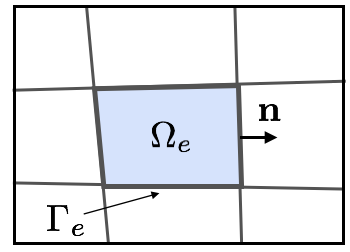
\includegraphics[width=1.5in]{figures/DG_domain.png}
\label{fig:spatial_discretization/dg_domain}}
\subfigure[Element $\Omega_e$]{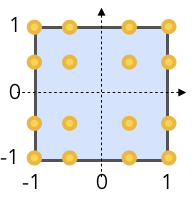
\includegraphics[width=1.5in]{figures/DG_element.png}
\label{fig:spatial_discretization/dg_element}}
\end{center}
\caption{The (a) global domain and (b) element ($N=3$) for the DG method.}
\label{fig:spatial_discretization/dg_method}
\end{figure}

To construct discrete approximations of continuous differential operators (e.g., gradient, divergence, or curl) with the DG method, we first must represent the state (solution) vector $\vec{Y}$ using a polynomial representation.  That is, we represent the state vector inside of each element $\Omega_e$ as
\be
\vec{Y}^{(e)}_N(\vec{x},t) = \sum_{i=1}^{M_N} \psi_i(\vec{x}) \vec{Y}^{(e)}_i(t),
\label{eq:spatial_discretization/dg_method}
\ee
where $\psi(\vec{x})$ are the known basis functions and $\vec{Y}^{(e)}_i(t)$ is the solution at each degree of freedom, which is time-dependent. The superscript $(e)$ represents the specific element we are working with, and $i=1,\ldots,M_N$ labels degrees of freedom inside each element $\Omega_e$.  Figure \ref{fig:spatial_discretization/dg_domain} shows a sample global domain, with one specific element $\Omega_e$ identified.  We then map the element from its physical space to the reference element presented in Fig.\ \ref{fig:spatial_discretization/dg_element}; in this particular example $M_N=(N+1)^2$ where $N=3$, which means we are using 3rd-degree polynomials in each direction (yielding 4th-order accuracy).  In general, $N$ need not be constant in each direction and so we can also write $M_N=(N_{\xi}+1)(N_{\eta}+1)$ in two dimensions or $M_N=(N_{\xi}+1)(N_{\eta}+1)(N_{\zeta}+1)$ in three dimensions, where $\xi$ is along the horizontal direction, $\eta$ along the vertical, and $\zeta$ coming out of the page. 

The attraction of using basis functions $\psi$ to represent the solution $\vec{Y}$ is that computing the gradient of $\vec{Y}$ now only requires applying the gradient operator directly to Eq.~\eqref{eq:spatial_discretization/dg_method}, which yields
\be
\nabla \vec{Y}^{(e)}_N(\vec{x},t) = \sum_{i=1}^{M_N} \nabla \psi_i(\vec{x}) \vec{Y}^{(e)}_i(t),
\label{eq:spatial_discretization/dg_method/gradient}
\ee
where we are able to construct $\grad \psi$ \emph{a priori} since we have chosen the basis functions $\psi$ not to depend on time.

\subsubsection{DG Representation of Conservation Laws}
To describe the DG method, let us describe how one would represent the divergence operator for the conservation law
\be
\diff{\vec{Y}}{t} + \nabla \cdot \Fvector = 0,
\label{eq:spatial_discretization/DG_divergence/conservation_law}
\ee
where, in two dimensions, the flux has components $\Fvector=F_x \wh{\vec{i}} + F_y \wh{\vec{j}}$.
To construct a discrete approximation to Eq.~\eqref{eq:spatial_discretization/DG_divergence/conservation_law}, we first multiply by a test function $\psi_i$ and integrate within each element $\Omega_e$ to arrive at the Galerkin problem statement: find $\vec{Y}^{(e)}_N \in L^2$ such that
\be
\inte \psi_i \diff{\vec{Y}^{(e)}_N}{t} d\Omega_e + \inte \psi_i \nabla \cdot \vecFe_N d\Omega_e= 0 \; \; \forall \; \; \psi \in L^2.
\label{eq:spatial_discretization/DG_divergence/conservation_law/discrete}
\ee
Using the product rule, the second term can be written as 
\be
\inte \psi_i \diff{\vec{Y}^{(e)}_N}{t} d\Omega_e + \inte \nabla \cdot \left( \psi_i \vecFe_N \right) d\Omega_e - \inte \nabla \psi_i \cdot \vecFe_N d\Omega_e= 0.
\label{eq:spatial_discretization/DG_divergence/conservation_law/discrete2}
\ee
Invoking the divergence theorem for the second term yields
\be
\inte \psi_i \diff{\vec{Y}^{(e)}}{t} d\Omega_e + \intb \psi_i \nvector \cdot \vecFe_N d\Gamma_e - \inte \nabla \psi_i \cdot \vecFe_N d\Omega_e= 0,
\label{eq:spatial_discretization/DG_divergence/conservation_law/discrete3}
\ee
where $\Gamma_e$ is the boundary of the element $\Omega_e$ and $\nvector$ is its outward pointing normal vector. We now need to fix the inconsistency of the second term above because it says that the solution along each element boundary $\Gamma_e$ is different from its neighbor since $\vecFe_N$ is allowed to be discontinuous across element boundaries (i.e., if $\vecFe_N \in C^1$ then no such inconsistency would exist).  To fix this, we introduce a numerical flux such that what flows from element $\Omega_e$ to its neighbor $\Omega_k$ is the negative of what flows from $\Omega_k$ into $\Omega_e$.  We represent this fix as follows
\be
\inte \psi_i \diff{\vec{Y}^{(e)}_N}{t} d\Omega_e + \intb \psi_i \nvector \cdot \Fvector^{(*,e)}_N d\Gamma_e - \inte \nabla \psi_i \cdot \vecFe_N d\Omega_e= 0,
\label{eq:spatial_discretization/DG_divergence/conservation_law/discrete4}
\ee
where $\Fvector^{(*,e)}_N$ is the numerical flux that takes into account the solution at $\Omega_e$ and all its neighbors $\Omega_k$ represented by $\Gamma_e$.  In two dimensions, we will have 4 face neighbors and in three dimensions we will have 6 face neighbors.  At this point, one is free to choose their favorite numerical flux just as one would do in the finite volume method (e.g., Rusanov, Roe, HLL, HLLC, etc.).  Note that it is the numerical flux term that couples all of the equations together; the rest of the terms are completely local within the element.

\subsubsection{Tensor Product Basis Functions}
In Eq.\ \eqref{eq:spatial_discretization/dg_method}, we have said very little about the basis functions $\psi$ and have written the approximation in so-called monolithic form whereby all the degrees of freedom within an element are written as one long vector of length $M_N$.  This way of representing Eq.\ \eqref{eq:spatial_discretization/dg_method} allows for a quick explanation of the DG method but does not illustrate how the method is constructed when tensor product basis functions are used.  In the case of tensor product basis functions, we rewrite $\psi$ (in 2D) as 
\[
\psi_i(\xi,\eta) = h_j(\xi) \otimes h_k(\eta),
\]
where $h$ are one-dimensional basis functions, $\otimes$ denotes the tensor (or Kronecker) product, and $j=1,\ldots N_{\xi}+1$, $k=1,\ldots,N_{\eta}+1$, and $i=j + (k-1) \left( N_{\xi}+1 \right)$. Using this strategy, we can now rewrite Eq.\ \eqref{eq:spatial_discretization/dg_method} as 
\be
\vec{Y}^{(e)}_N(\xi,\eta,t) = \sum_{i=1}^{N_{\xi}+1} \sum_{j=1}^{N_{\eta}+1} h_i(\xi) h_j(\eta) \vec{Y}^{(e)}_{ij}(t),
\label{eq:spatial_discretization/dg_method/tensor-product}
\ee
where we have written the approximation in terms of the reference element coordinates $(\xi,\eta)$ instead of the physical coordinates $(x,y)$.  The advantage of doing this is that the reference element and its coordinates never change, which means that we can use one set of basis functions for all of the elements in the mesh.  

Taking the gradient of Eq.\ \eqref{eq:spatial_discretization/dg_method/tensor-product} yields
\be
\diff{}{\vec{x}} \vec{Y}^{(e)}_N(\xi,\eta,t) = \diff{}{\vec{x}} \sum_{i=1}^{N_{\xi}+1} \sum_{j=1}^{N_{\eta}+1} h_i(\xi) h_j(\eta) \vec{Y}^{(e)}_{ij}(t)
\label{eq:spatial_discretization/dg_method/tensor-product/gradient}
\ee
where $\vec{x}$ can represent either $x$ or $y$.  Let us look at each component separately. Invoking the chain rule yields
\[
\diff{}{x}=\diff{}{\xi} \diff{\xi}{x} + \diff{}{\eta} \diff{\eta}{x}
\]
and
\[
\diff{}{y}=\diff{}{\xi} \diff{\xi}{y} + \diff{}{\eta} \diff{\eta}{y}
\]
where the metric terms $\diff{\vec{\xi}}{\vec{x}}$ need to be computed for each element in the mesh.
Using these we can now rewrite Eq.\ \eqref{eq:spatial_discretization/dg_method/tensor-product/gradient} for the $x$-derivative as 
\be
\diff{}{x} \vec{Y}^{(e)}_N(\xi,\eta,t) = \sum_{i=1}^{N_{\xi}+1} \sum_{j=1}^{N_{\eta}+1} \left( \diff{h_i(\xi)}{\xi}\diff{\xi}{x} h_j(\eta) + h_i(\xi) \diff{h_j(\eta)}{\eta}\diff{\eta}{x} \right) \vec{Y}^{(e)}_{ij}(t).
\label{eq:spatial_discretization/dg_method/tensor-product/x-deriv}
\ee
If we use the same polynomial order along $\xi$ and $\eta$ (call it $N$) then we can simplify Eq.\ \eqref{eq:spatial_discretization/dg_method/tensor-product/x-deriv} to
\be
\diff{}{x} \vec{Y}^{(e)}_N(\xi,\eta,t) = \sum_{i=1}^{N+1} \sum_{j=1}^{N+1} \left( dh_i \xi_x h_j + h_i dh_j \eta_x \right) \vec{Y}^{(e)}_{ij}(t).
\label{eq:spatial_discretization/dg_method/tensor-product/x-deriv2}
\ee
where $h$ is the basis function and $dh$ is its derivative, which are the same functions used along both directions $\xi$ and $\eta$; the index $(i,j)$ will account for which direction we are referring to.

This strategy readily extends to three-dimensions where we write the basis functions as 
\[
\psi_i(\xi,\eta,\zeta) = h_j(\xi) \otimes h_k(\eta) \otimes h_l(\zeta)
\]
with $j=1,\ldots N_{\xi}+1$, $k=1,\ldots,N_{\eta}+1$, $l=1,\ldots,N_{\zeta}+1$, and $i=j + (k-1) \left( N_{\xi}+1 \right) + (j-1)(k-1) \left( N_{\xi}+1 \right)\left( N_{\eta}+1 \right)$. Using this strategy we can rewrite Eq.\ \eqref{eq:spatial_discretization/dg_method} as 
\be
\vec{Y}^{(e)}_N(\xi,\eta, \zeta, t) = \sum_{i=1}^{N_{\xi}+1} \sum_{j=1}^{N_{\eta}+1} \sum_{k=1}^{N_{\zeta}+1} h_i(\xi) h_j(\eta) h_k(\zeta) \vec{Y}^{(e)}_{ijk}(t),
\label{eq:spatial_discretization/dg_method/tensor-product-3d}
\ee
where we have written the approximation in terms of the reference element coordinates $(\xi,\eta, \zeta)$ instead of the physical coordinates $(x,y,z)$. 

Taking the gradient of Eq.\ \eqref{eq:spatial_discretization/dg_method/tensor-product-3d} yields
\be
\diff{}{\vec{x}} \vec{Y}^{(e)}_N(\xi,\eta,\zeta,t) = \diff{}{\vec{x}} \sum_{i=1}^{N_{\xi}+1} \sum_{j=1}^{N_{\eta}+1} \sum_{k=1}^{N_{\zeta}+1} h_i(\xi) h_j(\eta) h_k(\zeta) \vec{Y}^{(e)}_{ijk}(t).
\label{eq:spatial_discretization/dg_method/tensor-product-3d/gradient}
\ee
Taking each component separately and invoking the chain rule yields
\[
\diff{}{x}=\diff{}{\xi} \diff{\xi}{x} + \diff{}{\eta} \diff{\eta}{x} + \diff{}{\zeta} \diff{\zeta}{x},
\]
\[
\diff{}{y}=\diff{}{\xi} \diff{\xi}{y} + \diff{}{\eta} \diff{\eta}{y} + \diff{}{\zeta} \diff{\zeta}{y},
\]
and
\[
\diff{}{z}=\diff{}{\xi} \diff{\xi}{z} + \diff{}{\eta} \diff{\eta}{z} + \diff{}{\zeta} \diff{\zeta}{z},
\]
where the metric terms $\diff{\vec{\xi}}{\vec{x}}$ need to be computed for each element in the mesh.
Using these we can now rewrite Eq.\ \eqref{eq:spatial_discretization/dg_method/tensor-product-3d/gradient} for the $x$-derivative as follows
\begin{eqnarray}
&& \diff{}{x} \vec{Y}^{(e)}_N(\xi,\eta,t) = \\ 
&& \sum_{i=1}^{N_{\xi}+1} \sum_{j=1}^{N_{\eta}+1} \sum_{k=1}^{N_{\zeta}+1} \left( \diff{h_i(\xi)}{\xi}\diff{\xi}{x} h_j(\eta) h_k(\zeta) + h_i(\xi) \diff{h_j(\eta)}{\eta}\diff{\eta}{x} h_k(\zeta) + h_i(\xi) h_j(\eta) \diff{h_k(\zeta)}{\zeta}\diff{\zeta}{x} \right) \vec{Y}^{(e)}_{ijk}(t) \nonumber .
\label{eq:spatial_discretization/dg_method/tensor-product-3d/x-deriv}
\end{eqnarray}
If we use the same polynomial order along $\xi$, $\eta$, and $\zeta$ then we can simplify Eq.\ \eqref{eq:spatial_discretization/dg_method/tensor-product-3d/x-deriv} as follows
\be
\diff{}{x} \vec{Y}^{(e)}_N(\xi, \eta, \zeta, t) = \sum_{i=1}^{N+1} \sum_{j=1}^{N+1} \sum_{k=1}^{N+1} \left( dh_i \xi_x h_j h_k + h_i dh_j h_k \eta_x + h_i h_j dh_k \zeta_x\right) \vec{Y}^{(e)}_{ijk}(t).
\label{eq:spatial_discretization/dg_method/tensor-product-3d/x-deriv2}
\ee
where the index $(i,j,k)$ will account for which direction we are referring to.

\subsection{Time-Discretization Methods}\label{s:timestepping}

\subsubsection{Additive Runge-Kutta IMEX Methods}
In order to circumvent the time-step restriction due to the fast moving acoustic waves, we will rely on implicit-explicit (IMEX) methods. For the LES model, if the aspect ratio of the horizontal to vertical grid spacing is near unity, it will be beneficial to use fully 3D-IMEX methods.  For the global atmospheric model with large aspect ratios of grid elements, we will use 1D-IMEX methods in which the time-integrator is fully explicit in the horizontal direction (HE) and implicit in the vertical direction (so-called HEVI schemes).

We propose to use a general family of additive Runge-Kutta methods (ARK) methods for both the 1D and 3D IMEX approaches (see, e.g., \citet{giraldo:2013} for 1D and 3D-IMEX methods based on ARKs). Note that adding fully-implicit Runge-Kutta (IRK) methods to the 3D-IMEX approach is quite trivial so this can be included as an option. Fully-implicit methods have no time-step restriction with respect to stability.

To get a sense of how the ARK approach works, let us partition the total tendency 
%\hl{[Note: please avoid using ``right-hand side'' as a term here and in the code. In the atmospheric and oceanic sciences, people understand it to mean something different. Tendency is unambiguous.]} \hl{[Frank Response: Even when referring to the direction of a specific equation? How do you propose I refer to the RHS of the equation below?]}\textcolor{red}{[]TS: Of course, RHS when referring to a specific equation is fine, and this is how I edited this text. Just not as a generic name, e.g., for tendencies, which invites confusion.]} 
$\vec{\mathcal{T}}$ on the right-hand side of Eq.~\eqref{e:eom_compact}, 

\comment{
\[
\Tvector = - \nabla \cdot \Fvector + \vec{\mathcal{S}} = \Tvector_N(\qvector) + \Tvector_L(\qvector),
\]
into nonlinear $\Tvector_N(\qvector)$ and linear $\Tvector_L(\qvector)$ parts. The stiffness due to grid spacing, acoustic waves, or fast sources is contained in $\Tvector_L(\qvector)$.  This then allows us to write the semi-discrete form (in space) as follows
}

\[
\Tvector = - \nabla \cdot \Fvector + \vec{\mathcal{S}} = \Tvector_{\mathrm{fastest}} + \Tvector_{\mathrm{fast}} + \Tvector_{\mathrm{dynamical}} + \Tvector_{\mathrm{slow}},
\]
which has been partitioned into four process speeds with $\Tvector_\mathrm{fastest}$ containing the fastest waves in the system including those responsible for the stiffness due to grid spacing, acoustic waves, and fast sources.  This then allows us to write the semi-discrete form (in space) as follows
\be
\difft{\qvector}{t} = \Tvector_\mathrm{fastest} + \Tvector_\mathrm{fast} + 
\Tvector_\mathrm{dynamical} + \Tvector_\mathrm{slow}.
\label{eq:IMEX}
\ee
\hl{[Below you already assume that $\Tvector_\mathrm{fastest}$ is linear. This needs to be clearer here. In other words, our fastest fluxes in the abstract model formulation were not necessarily linear, but here we already assume linearity, it seems.]} To discretize the equations in time, we first compute the stage values
\comment{
\be
\qstage^{(i)}=\qvector^n + \Delta t \sum_{j=0}^{i-1} \left( a_{ij} \Tvector_N(\qstage^{(j)}) \right) + \Delta t \sum_{j=0}^{i} \left( \wt{a}_{ij} \Tvector_L(\qstage^{(j)}) \right)
\label{eq:IMEX/stages}
\ee
}
\begin{eqnarray}
\qstage^{(i)}=&& \qvector^n + \Delta t \sum_{j=0}^{i} \left( a^{\mathrm{fastest}}_{ij} \Tvector_{\mathrm{fastest}}(\qstage^{(j)}) \right) + \Delta t \sum_{j=0}^{i-1} \left( {a}^{\mathrm{fast}}_{ij} \Tvector_{\mathrm{fast}}(\qstage^{(j)}) \right) \nonumber \\
&+&  \Delta t \sum_{j=0}^{i-1} \left( {a}^{\mathrm{dynamical}}_{ij} \Tvector_{\mathrm{dynamical}}(\qstage^{(j)}) \right) + \Delta t \sum_{j=0}^{i-1} \left( {a}^{\mathrm{slow}}_{ij} \Tvector_{\mathrm{slow}}(\qstage^{(j)}) \right)
\label{eq:IMEX/stages}
\end{eqnarray}
with $i=1,\ldots,s$ representing the $s$ stages, $\qstage^{(0)}=\qvector^n$ (where $\qvector^n$ is the solution vector at the current time), and $a$, are the coefficients of the partitioned Butcher tableau (see, e.g., \citet{constantinescu:2007, constantinescu:2007}). \hl{[Are we evaluating, e.g., even the slowest components at each stage $j$, with the same number of stages as the faster components? And how are the $a$'s different for the faster and slower components? I don't see how the sub- and superstepping comes about here.]} 
\fxg{We still need to work out the Butcher tableau but, yes, there are stage values for all components except that for the slower modes some rows of $a$ are zero and so are skipped. But we need to write them together for mathematical rigor.}
The solution at time $n+1$ is obtained from
\be
\qvector^{n+1}=\qvector^n + \Delta t \sum_{i=0}^{s} \left( b_i \vec{\mathcal{T}}(\qstage^{(i)}) \right).
\label{eq:IMEX/update}
\ee
So far we have defined a diagonally-implicit Runge-Kutta (DIRK) method \citep{alexander:1977,butcher:1981a,ascher:1997,boscarino:2009}.  To make the DIRK more efficient, we impose the restriction that all diagonal values $\wt{a}_{ii}$ are constant. This allows one construction of the matrix problem that does not change across stage values.  This we now refer to as singly-diagonally-implicit Runge-Kutta (SDIRK).

Rearranging Eq.\ \eqref{eq:IMEX/stages} as follows
\begin{eqnarray}
\qstage^{(i)} - {a}^{\mathrm{fastest}}_{ii} \Tvector_{\mathrm{fastest}}(\qstage^{(i)}) & = & \qvector^n + 
\Delta t \sum_{j=0}^{i-1} \left( {a}^{\mathrm{fast}}_{ij} \Tvector_{\mathrm{fast}}(\qstage^{(j)}) \right)  \label{eq:IMEX/stages2} \\
&+&  \Delta t \sum_{j=0}^{i-1} \left( {a}^{\mathrm{dynamical}}_{ij} \Tvector_{\mathrm{dynamical}}(\qstage^{(j)}) \right) + \Delta t \sum_{j=0}^{i-1} \left( {a}^{\mathrm{slow}}_{ij} \Tvector_{\mathrm{slow}}(\qstage^{(j)}) \right) 
\nonumber 
\end{eqnarray}
reveals the implicit nature of the problem since both terms on the left contain $\qstage^{(i)}$. To avoid a nonlinear solution procedure, we now linearize the fastest waves which allows us to write \hl{[This is just assumed here, i.e., there is an implicit assumption that fastest only contains linear components. Need to make this clearer.]} Eq. \eqref{eq:IMEX/stages2} as follows
\comment{
\be
\left( \vec{I} - \wt{a}_{ii} \Tvector_{L} \right) \qstage^{(i)} = \qvector^n + \Delta t \sum_{j=0}^{i-1} \left( a_{i,j} \Tvector_N(\qstage^{(j)}) \right) + \Delta t \sum_{j=0}^{i-1} \left( \wt{a}_{ij} \Tvector_L(\qstage^{(j)}) \right).
\label{eq:IMEX/stages3}
\ee
}
\begin{eqnarray}
\left( \vec{I} - {a}^{\mathrm{fastest}}_{ii} \Tvector_{\mathrm{fastest}} \right) \qstage^{(i)} & = & \qvector^n + 
\Delta t \sum_{j=0}^{i-1} \left( {a}^{\mathrm{fast}}_{ij} \Tvector_{\mathrm{fast}}(\qstage^{(j)}) \right) 
\\
&+&  \Delta t \sum_{j=0}^{i-1} \left( {a}^{\mathrm{dynamical}}_{ij} \Tvector_{\mathrm{dynamical}}(\qstage^{(j)}) \right) + \Delta t \sum_{j=0}^{i-1} \left( {a}^{\mathrm{slow}}_{ij} \Tvector_{\mathrm{slow}}(\qstage^{(j)}) \right) \nonumber
\label{eq:IMEX/stages3}
\end{eqnarray}
Letting $\vec{A}=\vec{I} - {a}^{\mathrm{fastest}}_{ii} \Tvector_{\mathrm{fastest}}$, $\vec{X}=\qstage^{(i)}$, and $\mathcal{B}$ the right-hand side of Eq.\ \eqref{eq:IMEX/stages3} allows us to write the final linear system 
\[
\vec{A} \vec{X} = \mathcal{B}.
\]
We can solve this linear system using, e.g., Krylov subspace methods such as GCR or GMRES (we cannot use conjugate gradient since the system is hyperbolic and therefore is not symmetric positive-definite in the current form). ARK of order $\order(\Delta ^k)$ for $k=2,\ldots,5$ are planned (which are roughly of order $k=s-1$ where $s$ denotes the number of stages.

\subsubsection{Linear and Nonlinear Splitting}
 To understand the specifics of the IMEX implementation requires a precise definition of the operators given in Eq.\ \eqref{eq:IMEX}. In what follows, we describe the splitting into the fastest processes, which are handled implicitly and are assumed to be linear, and the remaining processes, which are handled explicitly but perhaps with substepping. 
 
 \subsubsection{3D-IMEX Approach}
 \label{sec:3D-IMEX/v1}
If the grid aspect ratio between the horizontal $\Delta_h$ and the vertical $\Delta_v$ is near unity, $\Delta_h/\Delta_v \approx 1$, the stiffness of the equations arises from the acoustic modes (i.e., sound waves), which travel along all three spatial dimensions. For this situation we must extract the acoustic waves in all three spatial dimensions and treat them implicitly.  

Let us once again write the governing equations in semi-discrete (in space) form as follows 
\be
\difft{\qvector}{t} = \vec{\mathcal{T}}
\label{eq:3d-IMEX/T_operator}
\ee
where $\qvector$ is the state vector from section~\ref{s:abstract_model_formulation} and $\vec{\mathcal{T}} = - \nabla \cdot \Fvector + \Source$ is the total tendency.
\comment{\hl{[We need the entire state and tendencies in here, because we may want to treat boundary sources, microphysical sources etc. implicitly as well; also check signs here and in what follows, some seem wrong]}}
\comment{
\begin{equation}
 \vec{\mathcal{T}}(\qvector)=- \left( \begin{array}{c}
 \nabla \cdot (\rho \vec{u} ) \\
 \nabla \cdot (\rho \vec{u} \otimes \vec{u} + p \vec{I}_3 ) + \rho \nabla \Phi \\
 \nabla \cdot ( (\rho \etotal + p) \vec{u} ) 
\end{array}
\right) + \vec{\mathcal{S}} + \text{\hl{other (e.g., diffusive) flux terms}}.
\label{eq:3d-IMEX/S_operator}
\end{equation}
}
\comment{
\hl{include sources in here too, and also the diffusive fluxes?  We can include all the diffusive fluxes and other source terms in the implicit part as long as we can linearize them.  However, if the Schur complement idea that I have been working on works out, then we would not be able to include the diffusive fluxes but the advantage is that the linear system is much smaller, better conditioned and symmetric positive-definite. I am working on sorting out all of the terms into this equation for this document.}
 }
 Next, we introduce, e.g., the following splitting: $\rho(\vec{x},t)=\rho_0(\vec{x}) + \rho'(\vec{x},t)$, 
 $p(\vec{x},t)=p_0(\vec{x}) + p'(\vec{x},t)$, and 
 $E(\vec{x},t)=E_0(\vec{x}) + E'(\vec{x},t)$ where $E=\rho \etotal$, $E_0=\rho_0 \etotal_0$, and the terms $\vec{Y}'(\vec{x},t)=\vec{Y}(\vec{x},t)-\vec{Y}_0(\vec{x})$ denote perturbation variables from the reference state 
 $\vec{Y}_0$, which is time-independent and may be hydrostatically and/or geostrophically balanced. For a geostrophically balanced reference state, we would also need to split the velocities as follows $\vec{u}(\vec{x},t)=\vec{u}_0(\vec{x}) + \vec{u}'(\vec{x},t)$.
 \comment{\hl{[This seems to assume a reference state at rest. Do we always assume that? If so, would be good to state.]}
 \hl{[Frank Response: Addressed this.]} \textcolor{red}{TS: Not quite my point. Yes, the reference state is time-independent. But you additionally seem to assume that it is at rest, i.e, the reference velocity is zero (there is no $u_0$ in the equations). Correct?}
 \hl{[Frank Response: Yes, we are assuming this here but is not strictly necessary to assume this.]}}

  \comment{
 construct the following linear representation of $\vec{\mathcal{T}}$ 
 \begin{equation}
 \vec{L}(\qvector)=- \left( \begin{array}{c}
 \nabla \cdot (\rho \vec{u} ) \\
 \nabla p'  + \rho' \nabla \Phi \\
 \nabla \cdot ( (E_0 + p_0) \vec{u} )
\end{array}
\right)
\label{eq:3d-IMEX/L_operator}
\end{equation}
}
 
 \comment{
 \hl{[This is not correct in the moist case, see the earlier sections. We might compute $p' = \rho_0 R_m T' + \rho' R_m T_0$, with temperature from thermodynamic state. However, should it not simply be $p’ = p-p_0$ with reference pressure $p_0$ consistent with thermodynamic state, so that we take care of the nonlinearity of the thermodynamics in the moist case?]}
 \hl{[Frank Response: I agree: I prefer to define the perturbation as $Y'=Y-Y_0$ for any field $Y$.]}
 }
 
 Introducing such a splitting into Eq.\ \eqref{eq:3d-IMEX/T_operator} allows us to decompose its right-hand side as follows
 \[
\Tvector= \Tvector_{\mathrm{fastest}} + \Tvector_{\mathrm{fast}} + \Tvector_{\mathrm{dynamical}} + \Tvector_{\mathrm{slow}}
\]
where $\Tvector_{\mathrm{fastest}}=-\nabla \cdot \Fvector_{\mathrm{fastest}} + \Source_{\mathrm{fastest}}$
 which must be linear with respect to $\qvector'$. 
 The crux of the IMEX formulation is the construction of the linear operator $\Tvector_{\mathrm{fastest}}$.  As a first approach, let us define this operator as follows:
 \[
 \Tvector_{\mathrm{fastest}}=-\nabla \cdot \left( \Fadv_{\mathrm{fastest}} + \Pvector_{\mathrm{fastest}} + \Fdiff_{\mathrm{fastest}} \right) + \Source_{\mathrm{fastest}}
 \]
 where we start with the fluxes given by Eqs.\ \eqref{e:adv_flux}--\eqref{eq:diff_flux} and write their linear representations as follows
 \begin{equation}
 \Fadv_{\mathrm{fastest}}=\left( \begin{array}{c}
 \rho \vec{u} \\
 \vec{0} \\
 \rho_0 e_0 \vec{u}\\
\vec{0}\\
\vec{0} \\
\vec{0}
\end{array}
\right), 
\Pvector_{\mathrm{fastest}}= \left( \begin{array}{c}
\vec{0} \\
p' \vec{I}_3 \\
p_0 \vec{u}\\
\vec{0} \\
\vec{0} \\
\vec{0} 
\end{array}
\right),
\Fdiff_{\mathrm{fastest}}=\left( \begin{array}{c}
 \rho_0 \vec{d}_{q_t} \\
 \rho_0 \vec{\tau}\\
 \rho_0 \vec{J} + \rho_0 \vec{D} \\
\rho_0 \vec{d}_{q_k}\\
\rho_0 \vec{d}_{q_{p, i}}\\
\rho_0 \vec{d}_{\chi_j}
\end{array}
\right)
\label{eq:fluxes_linear}
\end{equation}
which are linear with respect to $\rho'$, $\rho \vec{u}$ (and $\vec{u}$ by extension), and $(\rho \etotal - \rho_0 e_0)$.
\fxg{In principle, we can include the diffusive terms but there are vices and virtues to doing this. For one, we will not be able to extract a straightforward Schur complement (or at all).  Even without a Schur complement, we need to make the implicit solve dimension as small as possible. Using GCR or GMRES which require storing Arnoldi vectors for each iteration.  This will place a limit on the size of the problem that we can do on the GPU.  So the question is what do we gain from adding the diffusive fluxes.  Typically we are in the high Reynolds number regime so the stiffness will always be the acoustic waves.} \textcolor{red}{TS: Reynolds number is irrelevant here (because it is large). The problem lies with SGS turbulent fluxes we need to model, and they can be large. However, let's leave the diffusive fluxes out for now if that simplifies matters. They may not be crucial.}

The remaining term to linearize is the source vector \eqref{eq:source} which we now define
\be
\Source_{\mathrm{fastest}} = \left( \begin{array}{c}
 -\rho_0 C(q_t \rightarrow q_p) \\
 -2 \vec{\Omega} \times \rho\vec{u} - \rho' \nabla\Phi \\
 -\sum_{j\in\{v,l,i\}} (I_j + \Phi)  \rho_0 C(q_j \rightarrow q_p) - M \\
-\rho_0 C(q_k \rightarrow q_p, q_i)\\
\rho_0 C(q_k \rightarrow q_{p, i}) - \rho_0 C(q_{p, i} \rightarrow q_{p, j})\\
\rho_0 \mathcal{S}_{\chi_i}
\end{array}
\right).
\label{eq:source_linear}
\ee
\fxg{Need to look closer at the terms in the Source function to see what can be linearized.}
 With the $\Tvector_{\mathrm{fastest}}$ operator defined, we can then define the remaining nonlinear operator as $\Tvector - \Tvector_{\mathrm{fastest}}$.
 
 Using this splitting yields the maximum eigenvalue  the Jacobian operators  $\lambda^{\mathrm{remainder}}_{\max}=\widehat{\vec{n}} \cdot \vec{u} + c_s$ and 
 $\lambda^{\mathrm{fastest}}_{\max}= c_s$, where $c_s$ is the speed of sound \eqref{e:soundspeed} in moist air.
 
 \comment{
\subsubsection{3D-IMEX Approach: Version 2}
\label{sec:3D-IMEX/v2}
The advantage of using version 1 presented in Sec.\ \ref{sec:3D-IMEX/v1} is that we can construct the explicit solution of the governing equations and then view the implicit portion of the IMEX method as a correction to the explicit solution.  However, following this approach may cause the discrete form of the equations to lose hyperbolicity (see \cite{bispen:2017}).

To avoid this situation, we split the $\vec{\mathcal{T}}$ operator directly into a linear and nonlinear part:
\begin{equation}
 \vec{\mathcal{T}}(\qvector)=- \left( \begin{array}{c}
 0 \\
 \nabla \cdot (\rho \vec{u} \otimes \vec{u}) \\
 \nabla \cdot ( (E' + p') \vec{u} )
\end{array}
\right) 
+
\left( \begin{array}{c}
 \nabla \cdot (\rho \vec{u} ) \\
 \nabla p'  + \rho' \nabla \Phi \\
 \nabla \cdot ( (E_0 + p_0) \vec{u} )
\end{array}
\right).
\label{eq:3d-IMEX/S_operator/split}
\end{equation}
 Here, we have eliminated the reference pressure gradient and reference buoyancy due to, e.g., hydrostatic balance. With this approach, the maximum eigenvalue for the Jacobian operators are $\lambda^{(N)}_{\max}=2 \widehat{\vec{n}} \cdot \vec{u}$ and 
 $\lambda^{(L)}_{\max}= c_s$, where the superscripts (N) and (L) denote the operator that the eigenvalue is associated with.
}

\comment{
\subsubsection{1D-IMEX Approach}
\label{sec:1D-IMEX}
For grid aspect ratios $\Delta_h/\Delta_v \gg 1$, the stiffness of the equations will arise from the vertically propagating acoustic modes if the explicit CFL number will not be violated in the horizontal. For this situation, we only need to extract acoustic waves along the vertical direction and treat them implicitly.  Following a similar approach to version 1 for the 3D-IMEX method given in Sec.\ \ref{sec:3D-IMEX/v1}, we write \hl{[changed to notation that is standard in atmospheric sciences]}
\begin{equation}
 L(\qvector)=- \left( \begin{array}{c}
 \diff{}{z} (\rho w) \\
 \diff{p'}{z}  + (\rho' \nabla \Phi) \cdot \wh{k} \\
 \diff{}{z}  ( (E_0 + p_0) w)
\end{array}
\right)
\label{eq:1d-IMEX/L_operator}
\end{equation}
where $w$ denotes the velocity component along the vertical ($z$) direction with unit vector $\wh{k}$. With this operator defined, we can define $\vec{N}(\qvector)=\vec{\mathcal{T}}(\qvector) - \vec{L}(\qvector)$ and follow the procedure outlined in Sec.\ \ref{sec:3D-IMEX/v1}. 
}


\section{Topography}
Topography can be either built analitycal or by reading an external topography file. As of now, only {\bf NOAA based text files are being read} but the code will be ready to read DEM and {\tt NCDF} files as well. 
An example of high order grid built on the topography of the Monterey bay in California is shown in Figure \ref{fig:montereySurfaceGrid}. The high order grid is built so that the elements follow the geometric curvature. A detailed view of the curved high order elements is shown in Figure \ref{fig:gridDetailView}

\begin{figure}[htbp]
\centering
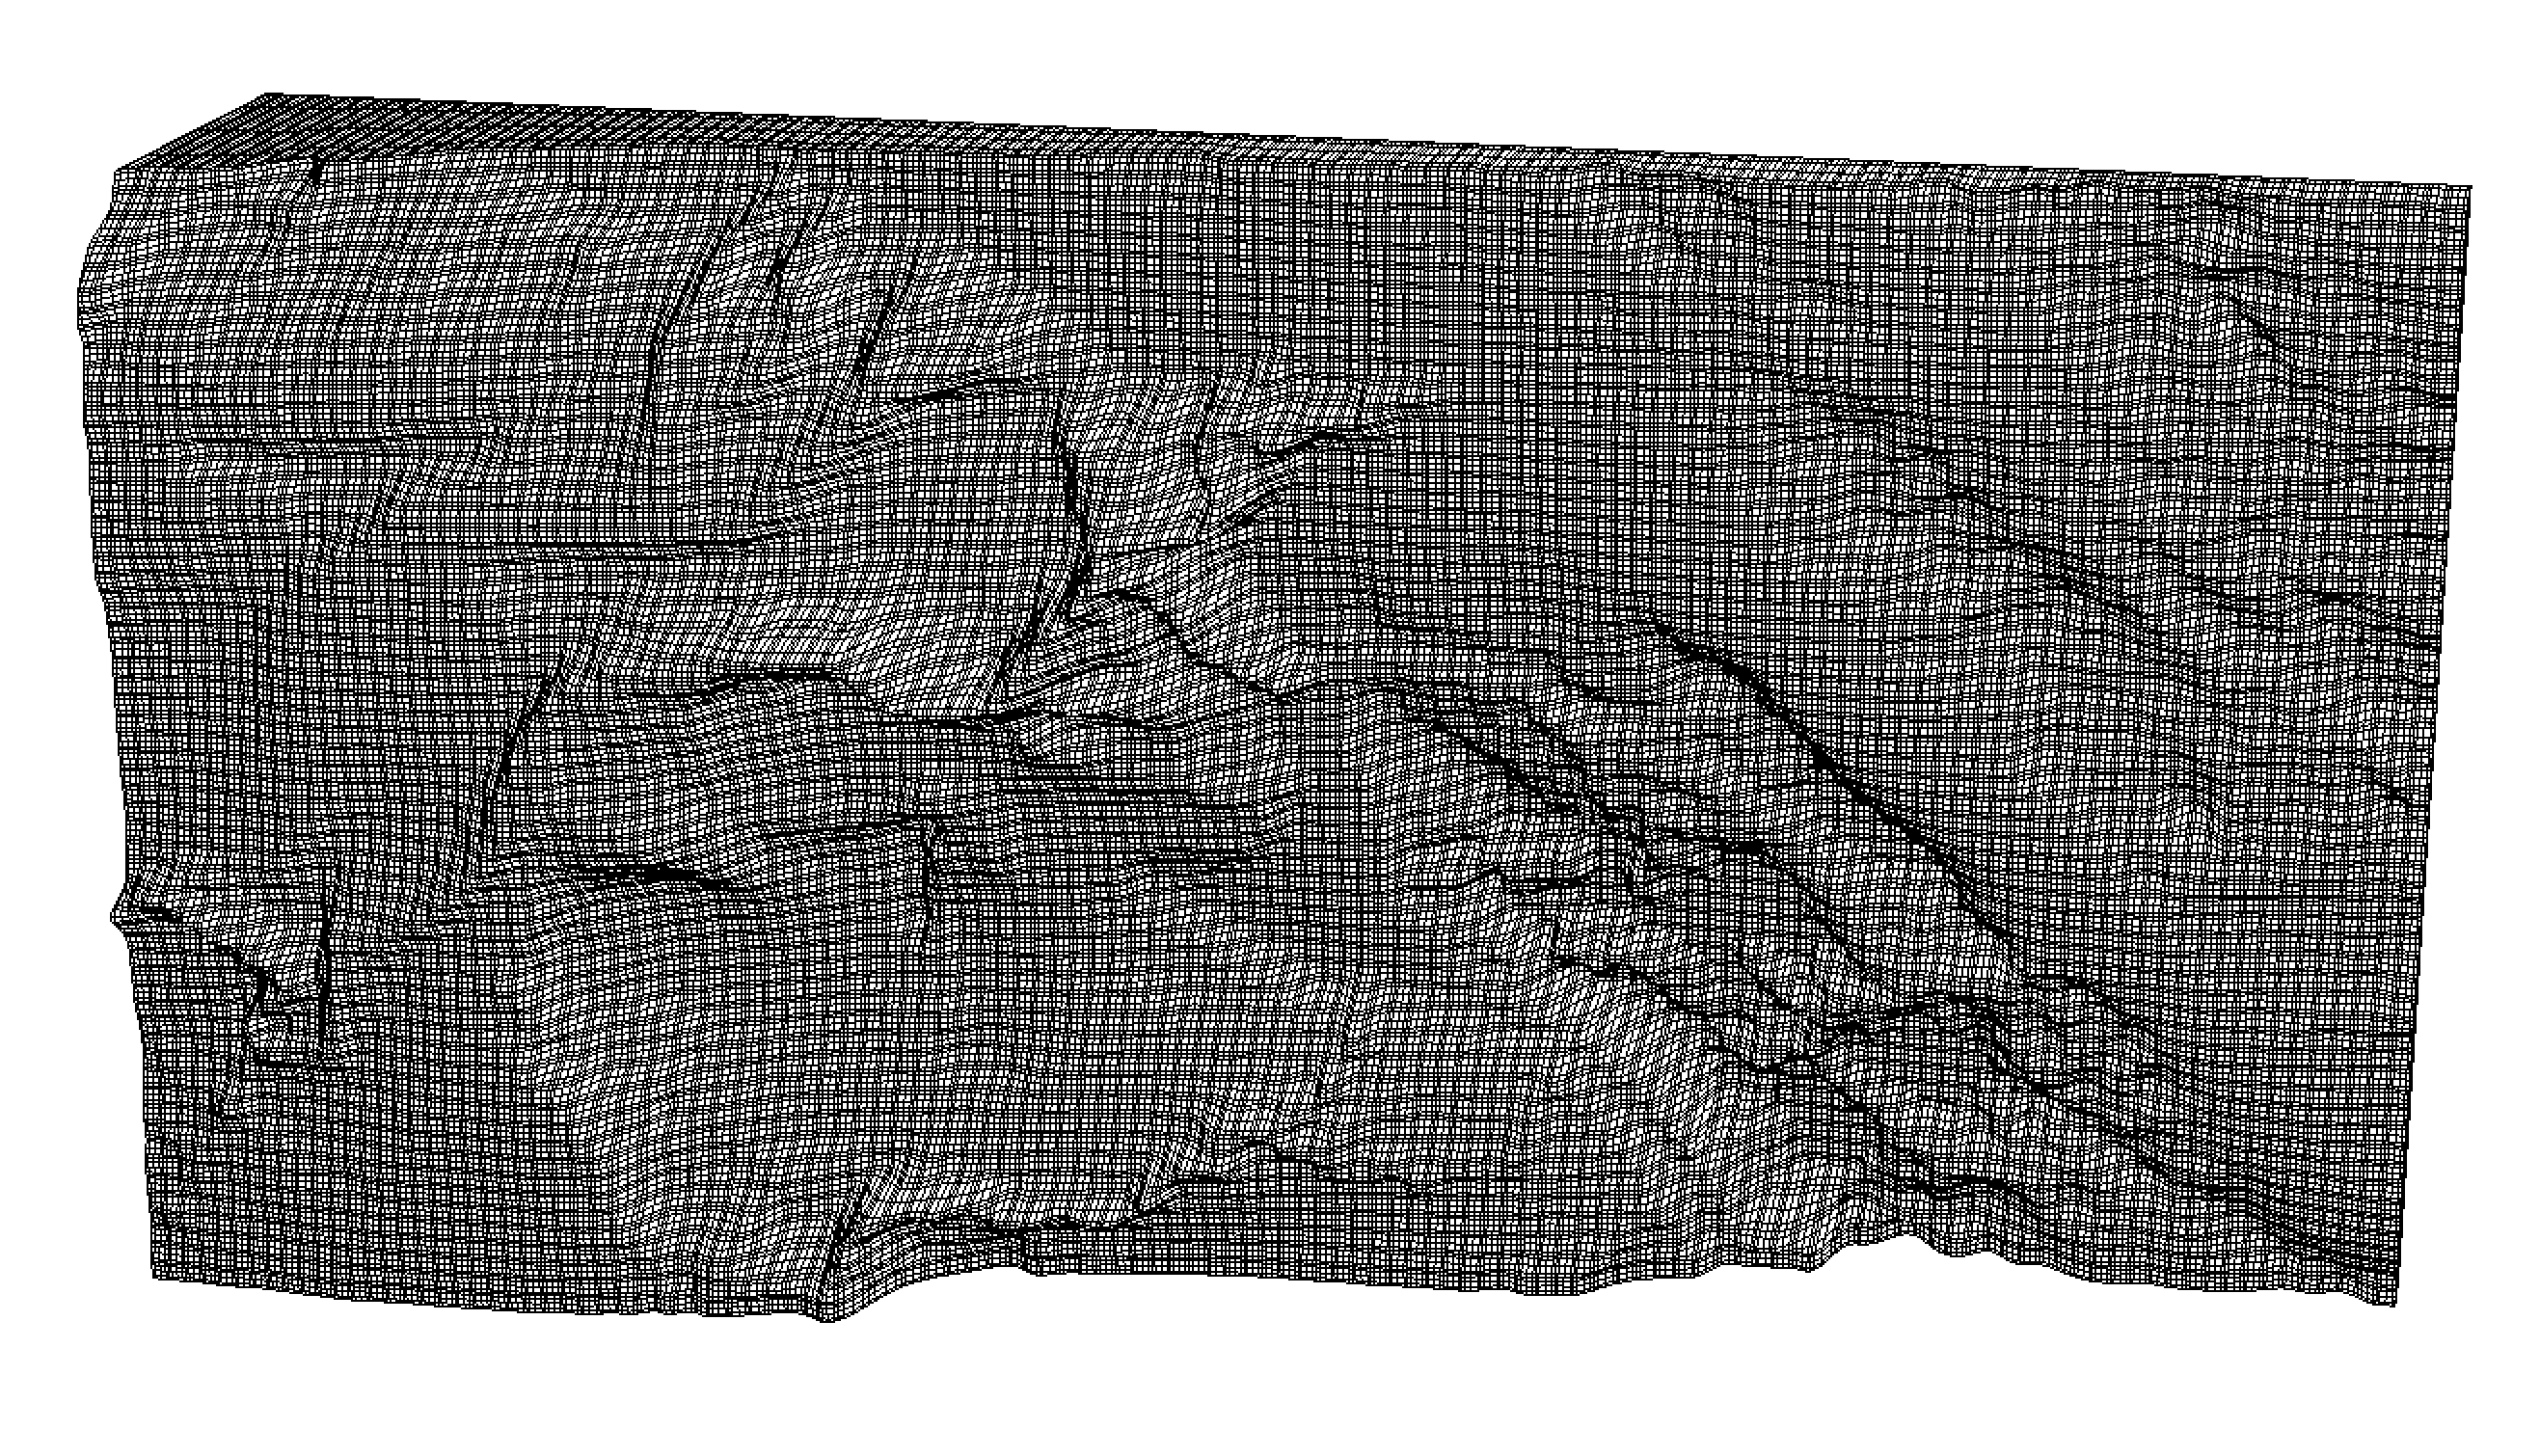
\includegraphics[width=\textwidth]{figures/monterey_with_grid.png}
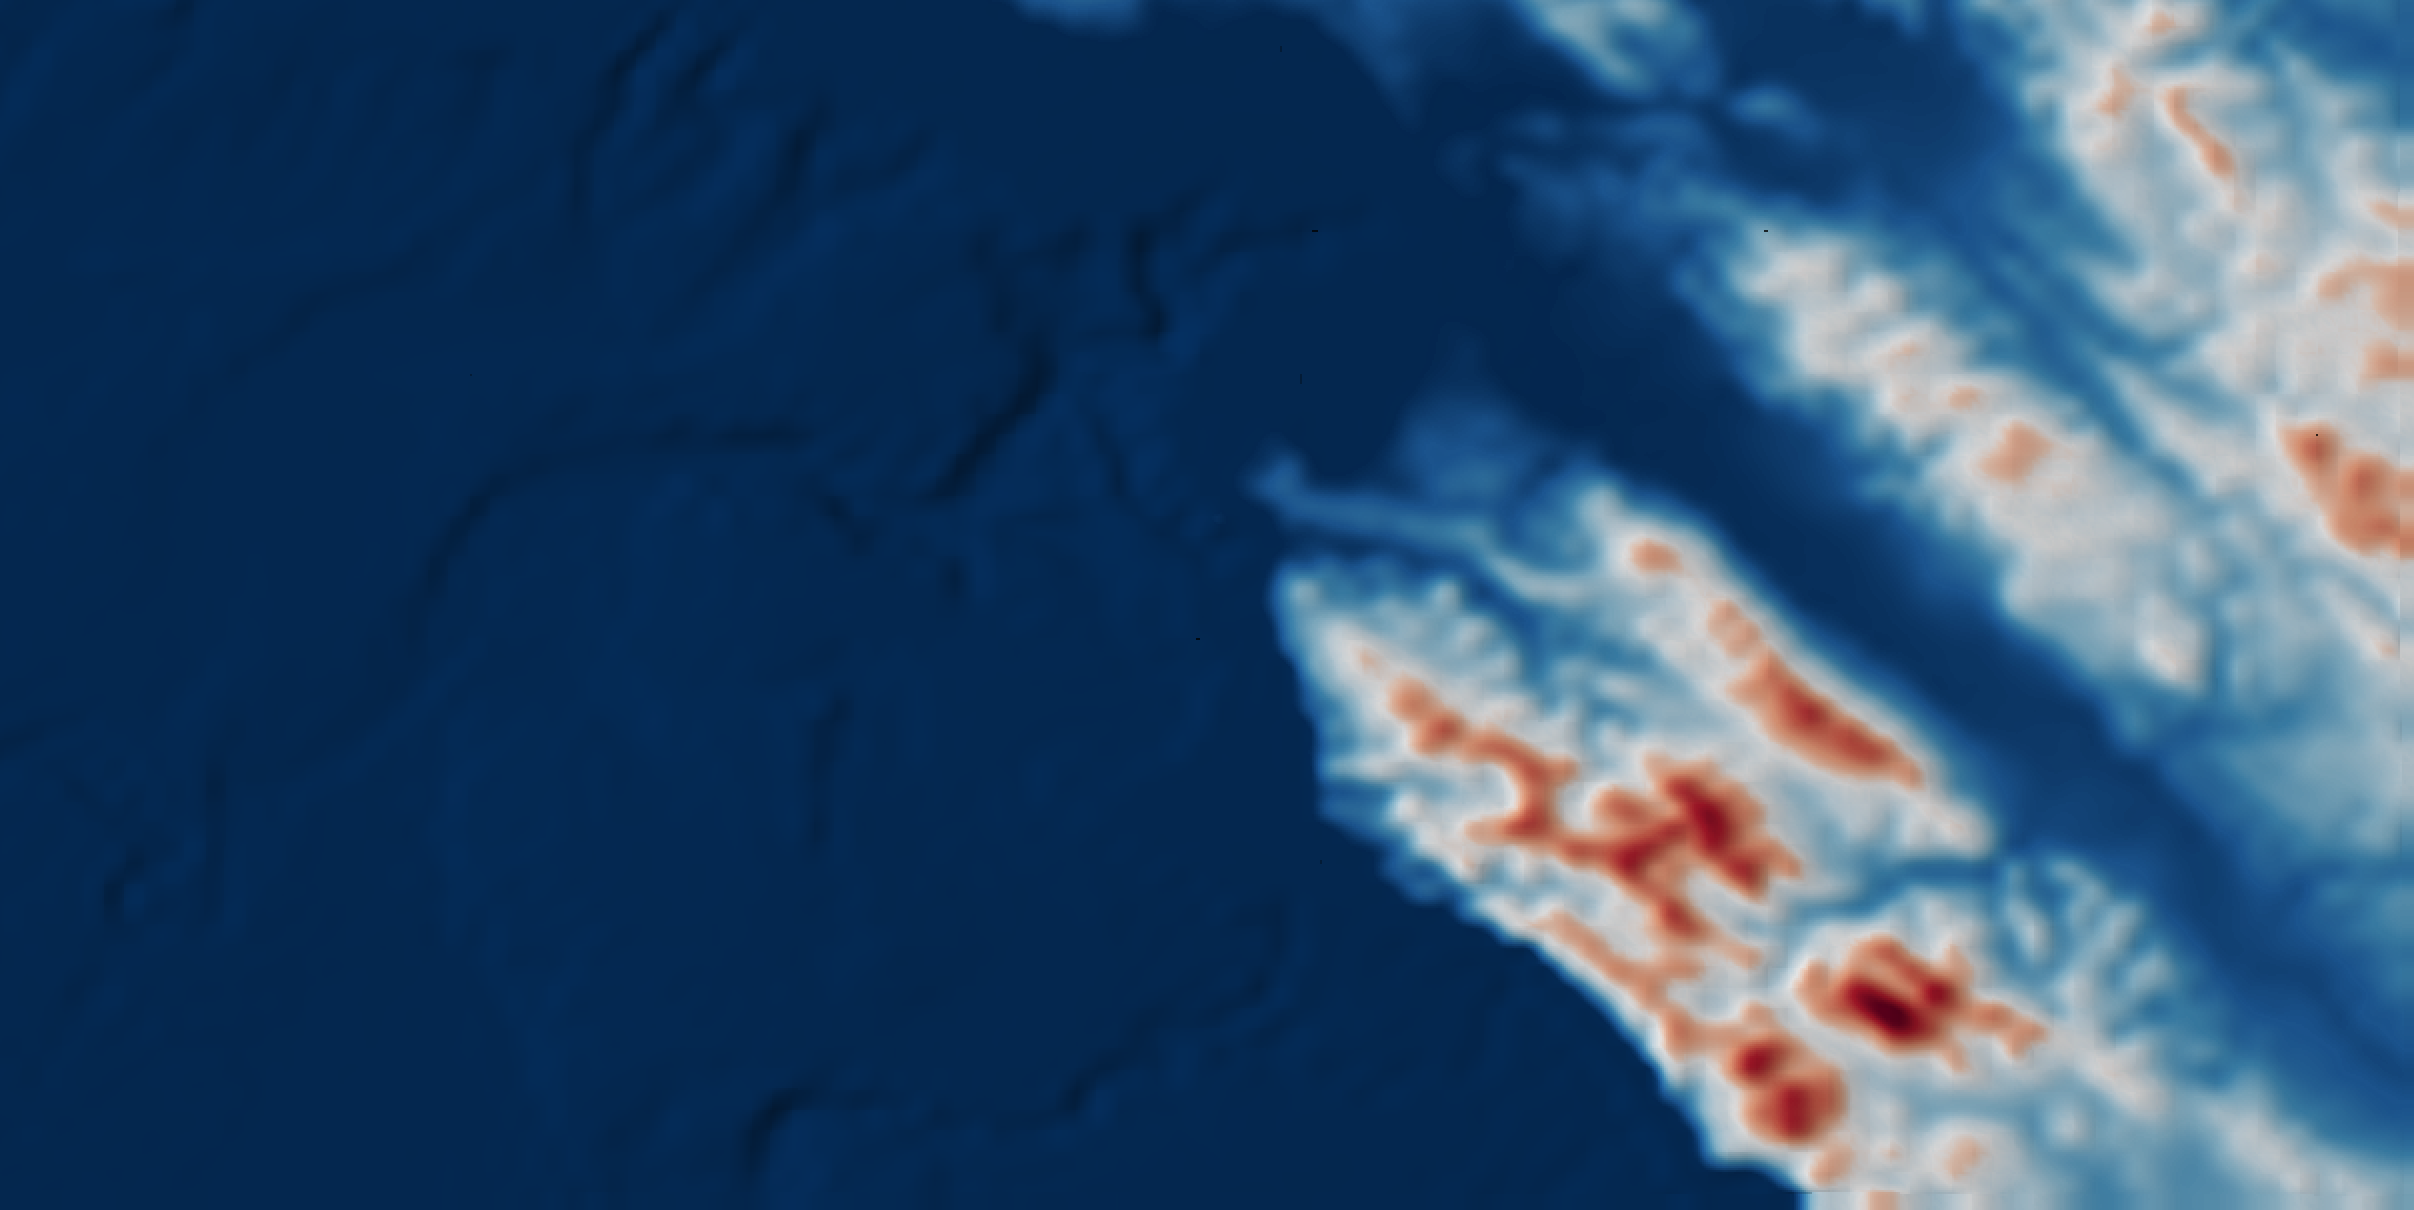
\includegraphics[width=\textwidth]{figures/monterey_colorscale.png}
\caption{Bottom view of the meshed Monterey Bay, California. The high order elements are visible in the top image whereas the topography is colored by its elevation in the bottom.}
\label{fig:montereySurfaceGrid}
\end{figure}

\begin{figure}[htbp]
\centering
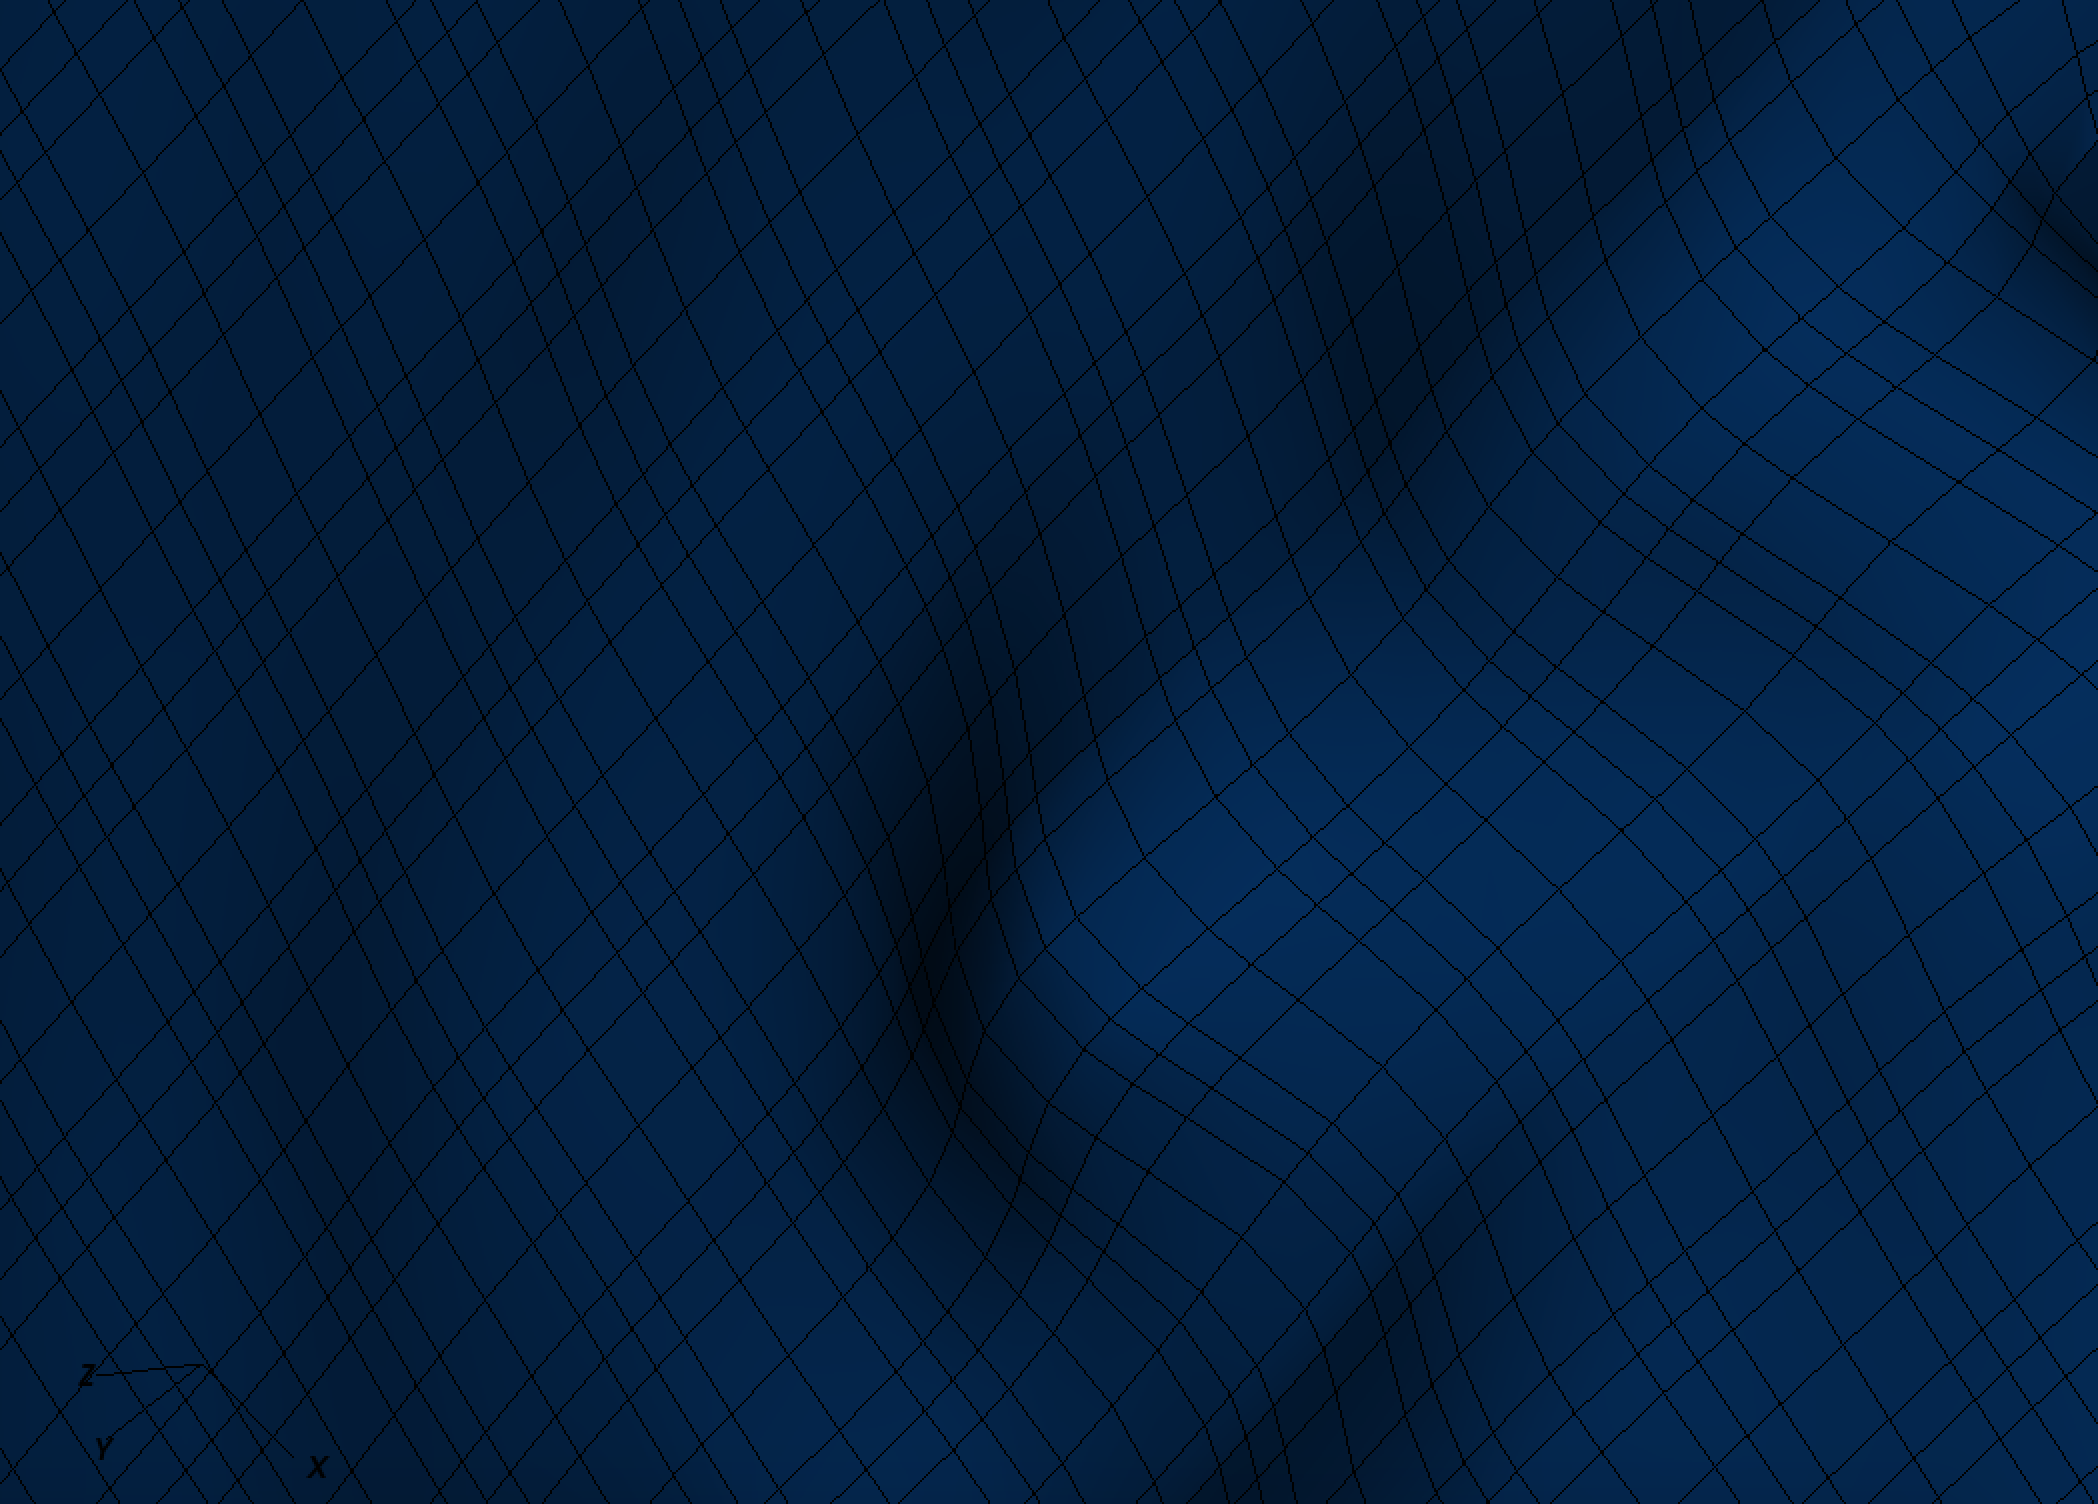
\includegraphics[width=\textwidth]{figures/GRID-detail.png}
\caption{A close view of the curved high order elements on the topography.}
\label{fig:gridDetailView}
\end{figure}

\section{Benchmarking the dynamical core (Dycore)}
\hl{STILL INCOMPLETE}
A set of benchmarks for dry and moist atmospheres are described in this section. The results presented in this document have been assessed against those presented in the literature. 

\hl{The grid reader should be enhanced to map the grid onto the sphere. As of now, the grid is read and mapped into a closed box only.}


\begin{enumerate}
        \item 2D/3D rising thermal bubble in a dry, neutrally stratified atmosphere. \citep{robert1993}.
        \item 2D density current \citep{strakaWilhelmson1993}.
        %\item 2D rising thermal bubble in a saturated atmosphere \citep{kurowskiEtAl2013}.
        \item pseudo 2D and 3D squall line \citep{gabersekGiraldoDoyle2012}
        \item Dynamics and chemistry of marine stratocumulus: Dycoms \citep{Stevens05a}.
\end{enumerate}

%%
\subsection{2D rising thermal bubble by Robert 1993}
\label{2dRTBtest}
This test is described \cite{robert1993}. It consists of a flow that is triggered by the thermal perturbation of a neutrally stratified atmosphere at initially uniform potential temperature $\theta_0 = 303$ K
and in hydrostatic equilibrium such that the pressure decreases with $z$ as:
\begin{equation}
\label{pressureDistrib}
p = p_{0}\left(1-\frac{g}{c_p{\theta_{0}}}z\right)^{c_p/R}.
\end{equation}
The domain $\Omega=[-5000,5000]\times[0,10000]\,{\rm m}^2$.
The perturbation is linear and defined as
\begin{equation}
 \Delta\theta = \left\{ \begin{array}{ll}
 \theta_c & \mathrm{if } r \leq a=50\,{\mathrm K}\\
 \theta_c e^{-(x - a)^2/\sigma^2} & \mathrm{if } r > a=50\,{\mathrm K}\\
\end{array} \right.
\label{eq:robertIni}
\end{equation}
where $r = \sqrt[]{(x-x_{c})^{2} + (z-z_{c})^{2}}$, $(x_c,z_c) = (500,260)\,{\rm m}$, $\sigma = 100$, and $\theta_c=0.5$ K.

\begin{figure}[htbp]
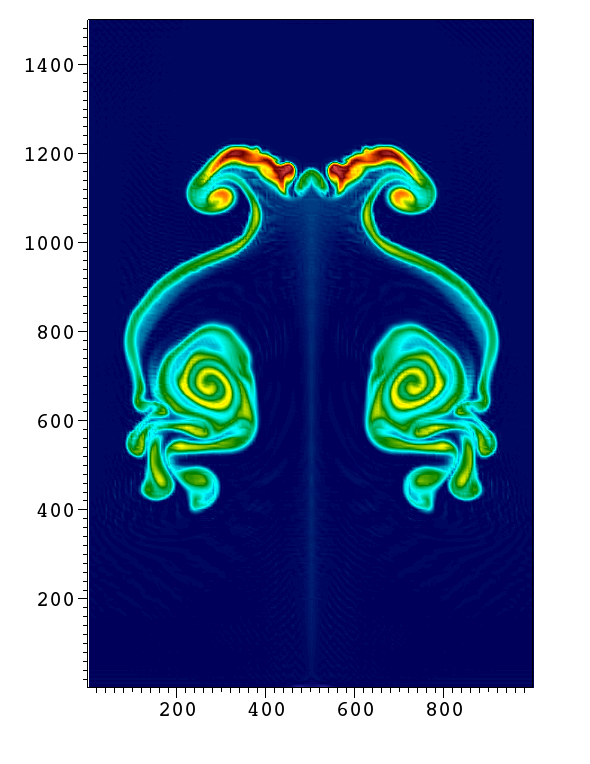
\includegraphics[width=\textwidth]{figures/RTB-Robert--smgo-5mX5m-1080s0000.png}
\caption{2D rising thermal bubble (Robert, 1993) stabilized via a constant coefficient Smagorinsky-Lilly SGS: Potential temperature, $\theta$, at $t=1080\,{\rm s}$. Grid resolution: $\Delta x = \Delta z = 5\,{\rm m}$.}
\label{fig:benchmarks/robert5msmago}
\end{figure}

\subsection{2D density current}
This test is described in \cite{strakaWilhelmson1993}. It consists of a flow that is triggered by the cold perturbation of a neutrally stratified atmosphere at initially uniform potential temperature $\theta_0 = 300$ K
and in hydrostatic equilibrium such that the pressure decreases with $z$ as:
\begin{equation}
\label{pressureDistrib}
p = p_{0}\left(1-\frac{g}{c_p{\theta_{0}}}z\right)^{c_p/R}.
\end{equation}
The domain $\Omega=[-25600,25600]\times[0,6400]\,{\rm m}^2$.
The perturbation is linear and defined as
\begin{equation}
 \Delta\theta = \left\{ \begin{array}{ll}
 0 & \mathrm{if } r > 1\,{\mathrm K}\\
 0.5 \theta_c \left(1 + \cos(\pi r) \right) \leq 1\,{\mathrm K}\\
\end{array} \right.
\label{eq:robertIni}
\end{equation}
where $r = \sqrt[]{(x-x_{c})^2/r_x^{2} + (z-z_{c})^{2}/r_z^2}$, $(x_c,z_c) = (0,4000)\,{\rm m}$, $(r_x, r_z) = (4000, 2000)\,{\rm m}$ and $\theta_c=-15$ K. The fully developed density current at $t=900\,{\rm s}$ simulated with a grid effective resolution of $25$ m in both spatial directions is shown in Figure \ref{fig:benchmarks/dc25msmago}.

\begin{figure}[htbp]
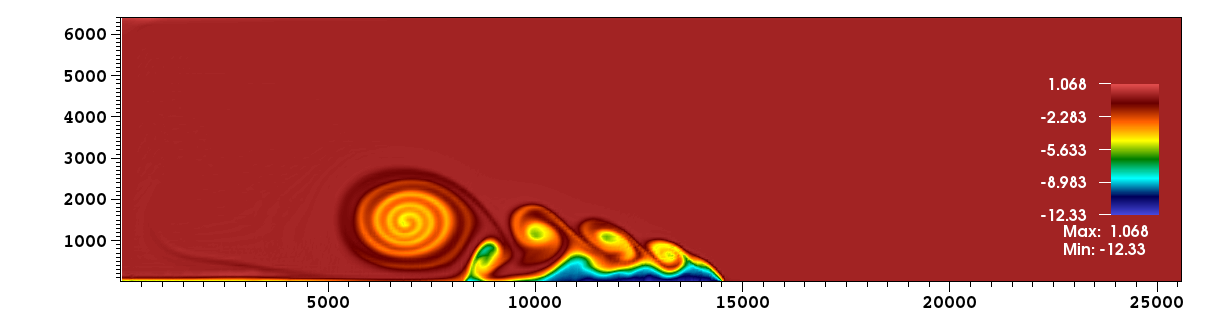
\includegraphics[width=1.2\textwidth]{figures/DC-smgo-25mx25m-900s0000.png}
\caption{2D density current stabilized via a constant coefficient Smagorinsky-Lilly SGS. Potential temperature, $\theta$, at $t=900\,{\rm s}$ (top) and at $t=1200\,{\rm s}$ (bottom). Grid resolution: $\Delta x = \Delta z = 25\,{\rm m}$.
}
\label{fig:benchmarks/dc25msmago}
\end{figure}


%%
\subsection{Rising thermal bubble in a saturated atmosphere}
\label{rtb3D}
The moist dynamics is tested by means of the saturated rising bubble test described in \cite{Pressel15a}. The initial conditions are setup as follows:

\begin{itemize}
\item Initialize dry atmosphere with uniform background $\theta_{ref} = 320$ K
\item Add thermal perturbation $\Delta \theta$ of radius $r=2$ km
\item Set a uniform total mixing ratio $q_t = 0.0192 \,{\rm kg/kg}$ and $q_l = q_i = 0.0\,{\rm kg/kg}$
\item Calculate the gas constants for moist air: 
\[\begin{array}{lcl}
R_{gas} &=& {\tt MoistThermodynamics.gas\_constant\_air(q_t, q_l, q_i)}\\
c_v     &=& {\tt MoistThermodynamics.cv\_m(q_t, q_l, q_i)}\\
c_p     &=& {\tt MoistThermodynamics.cp\_m(q_t, q_l, q_i)}\\
\end{array}
\]
\item  Compute $\theta$, $\rho$, and $T$ as if the background were dry:\\
    \[ \begin{array}{lcl}
  \theta &=& \theta_{ref} + \Delta\theta\\
 \pi & =& 1 - gz/(c_p\theta)\\
 \rho & = & p0/(R_{gas}\theta)\pi^(c_v/R_{gas})\\
 T   & = &\pi \theta
\end{array}\]

\item Add the contribution of moisture to the internal energy and recalculate $T$ and $P$, and obtain $e^{\rm tot}$ using the following {\tt MoistThermodynamics} functions:
\[\begin{array}{lcl}
I &=& {\tt MoistThermodynamics.internal_energy(T + T_0, q_t, q_l, q_i)}\\
T &=& {\tt MoistThermodynamics.air_temperature(I, q_t, q_l, q_i)}\\
P &=& {\tt MoistThermodynamics.air_pressure(T - T_0, \rho, q_t, q_l, q_i)}\\
e^{\rm tot} &=& {\tt MoistThermodynamics.total_energy(0.5\|{\bf u} \|^2, gz, T, q_t)}
\end{array}\]
\end{itemize}

%%
\subsection{3D squall line}
\label{sq3D}
\hl{ADD DESCRIPTION}
\begin{figure}[htbp]
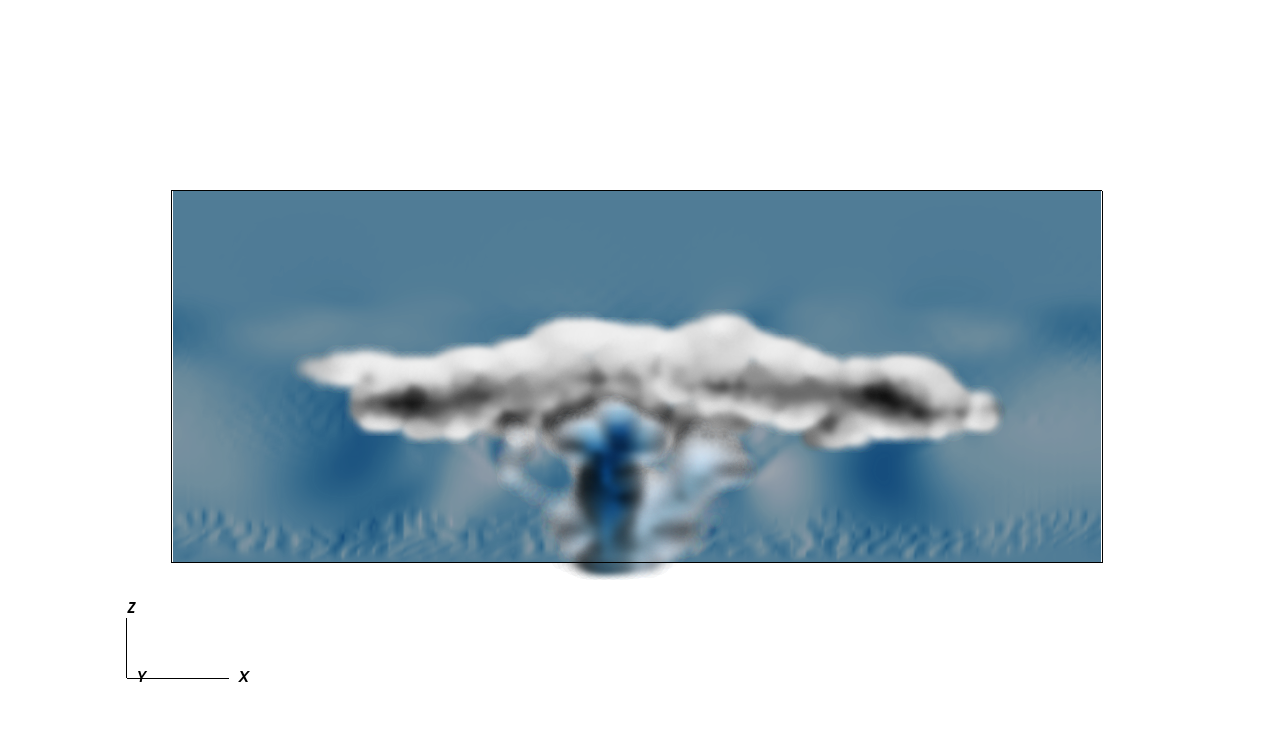
\includegraphics[width=1.2\textwidth]{figures/squall_working_warm_rain_frontal_view0028.png}
\caption{Front view of a fully developed squall line with precipitating rain. }
\label{fig:benchmarks/squall1}
\end{figure}


\subsection{External soundings}
External soundings can be read into the code for initialization purposes. The sounding requires the following format:

\begin{table*}[t]
\centering
{\footnotesize
\caption[short]{Structure of sounding files for simulation initialization.}
\label{DeltaDefinitionsTable}
\begin{tabular*}{\textwidth}{ @{\extracolsep{\fill}} llllll}
\hline
\hline
z (m) & $\theta_v$ (K) & $q_{tot}$ $\rm {kg/kg}$ & $u$ (m/s) & $v$ (m/s) & p (Pa)\\
0 & 300 & 14  & -2 & 0 & 100000\\
... & ... & ...  & ... & ... & ...\\
\hline

\hline
\hline
\end{tabular*}
}
\end{table*}


%\section{Tutorial of CliMa Kernels}
%\label{sec:tutorial}
%
%In \texttt{https://github.com/climate-machine/Canary.jl/tree/master/examples} the following three folders
%\begin{enumerate}
%    \item 1d$\_$kernels
%    \begin{itemize}
%        \item LDG1d
%        \item burger1d
%        \item swe1d
%    \end{itemize}
%    \item 2d$\_$kernels
%    \begin{itemize}
%        \item LDG2d
%        \item euler2d$\_$set3c
%        \item nse2d
%        \item nse2d$\_$sgs
%        \item swe2d
%    \end{itemize}
%    \item 3d$\_$kernels
%    \begin{itemize}
%        \item LDG3d
%        \item euler3d$\_$set3c
%        \item nse3d
%    \end{itemize}
%\end{enumerate}
%containing various sets of governing equations can be found. 
%
%In all the folders, the LDG files solve an elliptic equation (a Poisson equation) using the Local Discontinuous Galerkin (LDG) method.  The swe files solve the shallow water equations, the euler files solve the Euler equations using the conservation form with total energy, and the nse files solve the fully compressible Navier-Stokes equations (NSE) which are nothing more than the Euler equations with the viscous stresses solved via the LDG method.  All hyperbolic equations (burger, swe, and euler) use the discontinuous Galerkin (DG) method with a simple Rusanov flux with arbitrary order polynomial basis functions on tensor-product grids (1D line, 2D quads, and 3D hexahedra).
%
%All of these codes are structured in the same way.  Namely, at the bottom of each JL file there is a MAIN function that contains an initial condition and runs the program.  MAIN then calls the solver (e.g., in the case of Burgers equation, it calls the function BURGER, in the case of shallow water, it calls the SWE, in the case of Navier-Stokes, it calls the function NSE).  In turn, the solver function calls LOWSTORAGERK which is the time-integration loop and a proxy for any time-integrator that will be included in CliMa in the future (e.g., Additive Runge-Kutta methods for 1D-IMEX and 3D-IMEX).
%The heart of all these kernels is in the LOWSTORAGERK function which looks as follows
%\begin{algorithm}
%\label{alg:Time-Stepper}
%\begin{algorithmic}
%\Function{LOWSTORAGERK}{}
%\For{$step=1:nsteps$} \Comment go over time-steps
%\For{$s=1:length(RKstages)$} \Comment go over multi-stages
%\State 1ST$\_$ORDER$\_$OPERATOR \Comment use Alg. \ref{alg:first_order_operators}
%\If{viscosity>0}
%\State 2ND$\_$ORDER$\_$OPERATOR \Comment use Alg. \ref{alg:second_order_operators}
%\EndIf
%\State UPDATESOLUTION!() \Comment update the solution field q
%\EndFor 
%\EndFor
%\EndFunction
%\end{algorithmic}
%\end{algorithm}
%where it builds the first order operators and then, if required, the second order operators.  The function UPDATESOLUTION    updates the solution for the next time-step.  
%
%The first order operators are described in Alg.\ \ref{alg:first_order_operators} below.
%\begin{algorithm}
%\label{alg:first_order_operators}
%\begin{algorithmic}
%\Function{1ST$\_$ORDER$\_$OPERATOR}{}
%\State SENDDATA$\_$Q() \Comment non-blocking send of the data
%\State VOLUMERHS!() \Comment compute volume integral contribution to RHS
%\State RECEIVEDATA$\_$Q() \Comment non-blocking receive - for latency hiding
%\State FLUXRHS!() \Comment compute flux integral contribution to RHS
%\EndFunction
%\end{algorithmic}
%\end{algorithm}
%The SENDDATA and RECEIVEDATA functions exchange the information on the CPU and/or GPU and need to be called separately in order to overlap communication with computation (we send the data and while it is being sorted out, we compute the volume integrals which require no neighbor data).  Once we finish with the volume integrals (VOLUMERHS), we then wait to receive all the data (RECEIVEDATA$\_$Q) before we compute the flux integrals (FLUXRHS), which do require neighbor data. The "!" at the end of some of the function calls denotes that the state vector $q$ or $RHS$ is modified by that function.
%
%If second order differential operators are required (say for diffusion), then this is done after the 1st order operators as follows
%\begin{algorithm}
%\label{alg:second_order_operators}
%\begin{algorithmic}
%\Function{2ND$\_$ORDER$\_$OPERATOR}{}
%\State VOLUMEGRAD!() \Comment compute volume integral contribution to $\nabla q$
%\State FLUXGRAD!() \Comment compute flux integral contribution to $\nabla q$
%\State UPDATEGRAD!() \Comment update the solution to compute gridpoint $\nabla q$
%\State SENDDATA$\_$GRADQ() \Comment non-blocking send - for latency hiding
%\State VOLUMEDIV!() \Comment compute volume integral contribution to $\nabla \cdot (\nabla q)$
%\State RECEIVEDATA$\_$GRADQ() \Comment non-blocking receive - for latency hiding
%\State FLUXDIV!() \Comment compute flux integral contribution to $\nabla \cdot (\nabla q)$
%\EndFunction
%\end{algorithmic}
%\end{algorithm}
%Algorithm \ref{alg:second_order_operators} uses the local discontinuous Galerkin (LDG) method to construct 2nd order operators. We have used this approach for representing 2nd order operators because it is simpler to understand since it does so by first approximating the gradient of the function (VOLUMEGRAD and FLUXGRAD) and then computing the divergence of the gradient of the function (VOLUMEDIV AND FLUXDIV).  
%
%-------Bibliography
\bibliographystyle{agufull08}
\bibliography{Giraldo_refs,CLIMA-refs}

\end{document}
